% Options for packages loaded elsewhere
% Options for packages loaded elsewhere
\PassOptionsToPackage{unicode}{hyperref}
\PassOptionsToPackage{hyphens}{url}
\PassOptionsToPackage{dvipsnames,svgnames,x11names}{xcolor}
%
\documentclass[
  letterpaper,
  DIV=11,
  numbers=noendperiod]{scrreprt}
\usepackage{xcolor}
\usepackage{amsmath,amssymb}
\setcounter{secnumdepth}{5}
\usepackage{iftex}
\ifPDFTeX
  \usepackage[T1]{fontenc}
  \usepackage[utf8]{inputenc}
  \usepackage{textcomp} % provide euro and other symbols
\else % if luatex or xetex
  \usepackage{unicode-math} % this also loads fontspec
  \defaultfontfeatures{Scale=MatchLowercase}
  \defaultfontfeatures[\rmfamily]{Ligatures=TeX,Scale=1}
\fi
\usepackage{lmodern}
\ifPDFTeX\else
  % xetex/luatex font selection
\fi
% Use upquote if available, for straight quotes in verbatim environments
\IfFileExists{upquote.sty}{\usepackage{upquote}}{}
\IfFileExists{microtype.sty}{% use microtype if available
  \usepackage[]{microtype}
  \UseMicrotypeSet[protrusion]{basicmath} % disable protrusion for tt fonts
}{}
\makeatletter
\@ifundefined{KOMAClassName}{% if non-KOMA class
  \IfFileExists{parskip.sty}{%
    \usepackage{parskip}
  }{% else
    \setlength{\parindent}{0pt}
    \setlength{\parskip}{6pt plus 2pt minus 1pt}}
}{% if KOMA class
  \KOMAoptions{parskip=half}}
\makeatother
% Make \paragraph and \subparagraph free-standing
\makeatletter
\ifx\paragraph\undefined\else
  \let\oldparagraph\paragraph
  \renewcommand{\paragraph}{
    \@ifstar
      \xxxParagraphStar
      \xxxParagraphNoStar
  }
  \newcommand{\xxxParagraphStar}[1]{\oldparagraph*{#1}\mbox{}}
  \newcommand{\xxxParagraphNoStar}[1]{\oldparagraph{#1}\mbox{}}
\fi
\ifx\subparagraph\undefined\else
  \let\oldsubparagraph\subparagraph
  \renewcommand{\subparagraph}{
    \@ifstar
      \xxxSubParagraphStar
      \xxxSubParagraphNoStar
  }
  \newcommand{\xxxSubParagraphStar}[1]{\oldsubparagraph*{#1}\mbox{}}
  \newcommand{\xxxSubParagraphNoStar}[1]{\oldsubparagraph{#1}\mbox{}}
\fi
\makeatother

\usepackage{color}
\usepackage{fancyvrb}
\newcommand{\VerbBar}{|}
\newcommand{\VERB}{\Verb[commandchars=\\\{\}]}
\DefineVerbatimEnvironment{Highlighting}{Verbatim}{commandchars=\\\{\}}
% Add ',fontsize=\small' for more characters per line
\usepackage{framed}
\definecolor{shadecolor}{RGB}{241,243,245}
\newenvironment{Shaded}{\begin{snugshade}}{\end{snugshade}}
\newcommand{\AlertTok}[1]{\textcolor[rgb]{0.68,0.00,0.00}{#1}}
\newcommand{\AnnotationTok}[1]{\textcolor[rgb]{0.37,0.37,0.37}{#1}}
\newcommand{\AttributeTok}[1]{\textcolor[rgb]{0.40,0.45,0.13}{#1}}
\newcommand{\BaseNTok}[1]{\textcolor[rgb]{0.68,0.00,0.00}{#1}}
\newcommand{\BuiltInTok}[1]{\textcolor[rgb]{0.00,0.23,0.31}{#1}}
\newcommand{\CharTok}[1]{\textcolor[rgb]{0.13,0.47,0.30}{#1}}
\newcommand{\CommentTok}[1]{\textcolor[rgb]{0.37,0.37,0.37}{#1}}
\newcommand{\CommentVarTok}[1]{\textcolor[rgb]{0.37,0.37,0.37}{\textit{#1}}}
\newcommand{\ConstantTok}[1]{\textcolor[rgb]{0.56,0.35,0.01}{#1}}
\newcommand{\ControlFlowTok}[1]{\textcolor[rgb]{0.00,0.23,0.31}{\textbf{#1}}}
\newcommand{\DataTypeTok}[1]{\textcolor[rgb]{0.68,0.00,0.00}{#1}}
\newcommand{\DecValTok}[1]{\textcolor[rgb]{0.68,0.00,0.00}{#1}}
\newcommand{\DocumentationTok}[1]{\textcolor[rgb]{0.37,0.37,0.37}{\textit{#1}}}
\newcommand{\ErrorTok}[1]{\textcolor[rgb]{0.68,0.00,0.00}{#1}}
\newcommand{\ExtensionTok}[1]{\textcolor[rgb]{0.00,0.23,0.31}{#1}}
\newcommand{\FloatTok}[1]{\textcolor[rgb]{0.68,0.00,0.00}{#1}}
\newcommand{\FunctionTok}[1]{\textcolor[rgb]{0.28,0.35,0.67}{#1}}
\newcommand{\ImportTok}[1]{\textcolor[rgb]{0.00,0.46,0.62}{#1}}
\newcommand{\InformationTok}[1]{\textcolor[rgb]{0.37,0.37,0.37}{#1}}
\newcommand{\KeywordTok}[1]{\textcolor[rgb]{0.00,0.23,0.31}{\textbf{#1}}}
\newcommand{\NormalTok}[1]{\textcolor[rgb]{0.00,0.23,0.31}{#1}}
\newcommand{\OperatorTok}[1]{\textcolor[rgb]{0.37,0.37,0.37}{#1}}
\newcommand{\OtherTok}[1]{\textcolor[rgb]{0.00,0.23,0.31}{#1}}
\newcommand{\PreprocessorTok}[1]{\textcolor[rgb]{0.68,0.00,0.00}{#1}}
\newcommand{\RegionMarkerTok}[1]{\textcolor[rgb]{0.00,0.23,0.31}{#1}}
\newcommand{\SpecialCharTok}[1]{\textcolor[rgb]{0.37,0.37,0.37}{#1}}
\newcommand{\SpecialStringTok}[1]{\textcolor[rgb]{0.13,0.47,0.30}{#1}}
\newcommand{\StringTok}[1]{\textcolor[rgb]{0.13,0.47,0.30}{#1}}
\newcommand{\VariableTok}[1]{\textcolor[rgb]{0.07,0.07,0.07}{#1}}
\newcommand{\VerbatimStringTok}[1]{\textcolor[rgb]{0.13,0.47,0.30}{#1}}
\newcommand{\WarningTok}[1]{\textcolor[rgb]{0.37,0.37,0.37}{\textit{#1}}}

\usepackage{longtable,booktabs,array}
\usepackage{calc} % for calculating minipage widths
% Correct order of tables after \paragraph or \subparagraph
\usepackage{etoolbox}
\makeatletter
\patchcmd\longtable{\par}{\if@noskipsec\mbox{}\fi\par}{}{}
\makeatother
% Allow footnotes in longtable head/foot
\IfFileExists{footnotehyper.sty}{\usepackage{footnotehyper}}{\usepackage{footnote}}
\makesavenoteenv{longtable}
\usepackage{graphicx}
\makeatletter
\newsavebox\pandoc@box
\newcommand*\pandocbounded[1]{% scales image to fit in text height/width
  \sbox\pandoc@box{#1}%
  \Gscale@div\@tempa{\textheight}{\dimexpr\ht\pandoc@box+\dp\pandoc@box\relax}%
  \Gscale@div\@tempb{\linewidth}{\wd\pandoc@box}%
  \ifdim\@tempb\p@<\@tempa\p@\let\@tempa\@tempb\fi% select the smaller of both
  \ifdim\@tempa\p@<\p@\scalebox{\@tempa}{\usebox\pandoc@box}%
  \else\usebox{\pandoc@box}%
  \fi%
}
% Set default figure placement to htbp
\def\fps@figure{htbp}
\makeatother





\setlength{\emergencystretch}{3em} % prevent overfull lines

\providecommand{\tightlist}{%
  \setlength{\itemsep}{0pt}\setlength{\parskip}{0pt}}



 


\KOMAoption{captions}{tableheading}
\makeatletter
\@ifpackageloaded{bookmark}{}{\usepackage{bookmark}}
\makeatother
\makeatletter
\@ifpackageloaded{caption}{}{\usepackage{caption}}
\AtBeginDocument{%
\ifdefined\contentsname
  \renewcommand*\contentsname{Table of contents}
\else
  \newcommand\contentsname{Table of contents}
\fi
\ifdefined\listfigurename
  \renewcommand*\listfigurename{List of Figures}
\else
  \newcommand\listfigurename{List of Figures}
\fi
\ifdefined\listtablename
  \renewcommand*\listtablename{List of Tables}
\else
  \newcommand\listtablename{List of Tables}
\fi
\ifdefined\figurename
  \renewcommand*\figurename{Figure}
\else
  \newcommand\figurename{Figure}
\fi
\ifdefined\tablename
  \renewcommand*\tablename{Table}
\else
  \newcommand\tablename{Table}
\fi
}
\@ifpackageloaded{float}{}{\usepackage{float}}
\floatstyle{ruled}
\@ifundefined{c@chapter}{\newfloat{codelisting}{h}{lop}}{\newfloat{codelisting}{h}{lop}[chapter]}
\floatname{codelisting}{Listing}
\newcommand*\listoflistings{\listof{codelisting}{List of Listings}}
\makeatother
\makeatletter
\makeatother
\makeatletter
\@ifpackageloaded{caption}{}{\usepackage{caption}}
\@ifpackageloaded{subcaption}{}{\usepackage{subcaption}}
\makeatother
\usepackage{bookmark}
\IfFileExists{xurl.sty}{\usepackage{xurl}}{} % add URL line breaks if available
\urlstyle{same}
\hypersetup{
  pdftitle={Frontify Service},
  pdfauthor={Gary Newport},
  colorlinks=true,
  linkcolor={blue},
  filecolor={Maroon},
  citecolor={Blue},
  urlcolor={Blue},
  pdfcreator={LaTeX via pandoc}}


\title{Frontify Service}
\author{Gary Newport}
\date{2025-10-10}
\begin{document}
\maketitle

\renewcommand*\contentsname{Table of contents}
{
\hypersetup{linkcolor=}
\setcounter{tocdepth}{2}
\tableofcontents
}

\bookmarksetup{startatroot}

\chapter{Introduction and Goals}\label{introduction-and-goals}

\section{Overview}\label{overview}

Today Marcomms manage marketing and brand across the comapny, its
subsidiaries and affiliates. The IT systems employed within Marcoms have
organically grown over many years, with technologies chosen to meet
specific needs at the time rather than aligned to a technology strategy
or assessed on a strategic fitness level of the companies IT. Often
technology choices were made with a UK-first approach, and therefore
some of these solutions impair Marcoms when attempting to offer global
services within different territories. Some of these solutions have also
poor user experiences, which cause friction for those employed to use
these technologies on a day-to-day basis.

As a result, the companies marketing eco-system is disparate and poorly
integrated, with poor usability and lacking the ability to centralise
and manage brand and content globally.

The Marcoms vision is to start to unify services together, starting with
a common production platform where digital assets and brands can be
centrally managed and pushed out globally. Marcoms has selected a
third-party platform (Frontify) to deliver this capability.

\section{Goals}\label{goals}

The goal of this phase of the implementation is integrate Frontify with
the sales platform so that, we can replace Drag and Drop with this new
unified service. It is proposed to offer 2 separate solutions to the
sales platform users.

\begin{itemize}
\tightlist
\item
  A automated quick brochure generator that has a prescribed approach on
  how to present documents and images to the service.

  \begin{itemize}
  \tightlist
  \item
    Ideal generate a email quality brochure, so we can get to market
    quickly.
  \end{itemize}
\item
  A bespoke option which will allow the users to modify and manipulate
  the brochures within Frontify.

  \begin{itemize}
  \tightlist
  \item
    This will generate a print quality brochure, aimed at more selective
    clients, but will take longer and involve manual manipulation of the
    brochures content.
  \end{itemize}
\end{itemize}

There is also the option of performing both brochure operations if need
be.

\bookmarksetup{startatroot}

\chapter{Architectural Constraints}\label{architectural-constraints}

\section{Architectural Goals}\label{architectural-goals}

Integration Goals with Frontify Marketing material services:

\begin{itemize}
\tightlist
\item
  Standardise Brochure Generation:

  \begin{itemize}
  \tightlist
  \item
    Implement consistent methods for creating brochures.
  \end{itemize}
\item
  Standardise Data Integration, Reporting, and Export:

  \begin{itemize}
  \tightlist
  \item
    Ensure uniform approaches for data handling and reporting.
  \end{itemize}
\item
  Utilise Current Patterns for Gathering Usage Information:

  \begin{itemize}
  \tightlist
  \item
    Adopt existing methods to collect and analyze usage data.
  \end{itemize}
\item
  Reduce Brochure Generation Time:

  \begin{itemize}
  \tightlist
  \item
    Streamline processes to create brochures more quickly.
  \end{itemize}
\item
  Control Brochure Look and Feel with Marketing Templates:

  \begin{itemize}
  \tightlist
  \item
    Maintain a consistent design using marketing-approved templates.
  \end{itemize}
\end{itemize}

\section{Architectural Principles}\label{architectural-principles}

The proposed pattern architecture aligns to our current Group Technology
Principles as follows:

\begin{longtable}[]{@{}
  >{\raggedright\arraybackslash}p{(\linewidth - 6\tabcolsep) * \real{0.0036}}
  >{\raggedright\arraybackslash}p{(\linewidth - 6\tabcolsep) * \real{0.2473}}
  >{\raggedright\arraybackslash}p{(\linewidth - 6\tabcolsep) * \real{0.7309}}
  >{\raggedright\arraybackslash}p{(\linewidth - 6\tabcolsep) * \real{0.0182}}@{}}
\toprule\noalign{}
\begin{minipage}[b]{\linewidth}\raggedright
\#
\end{minipage} & \begin{minipage}[b]{\linewidth}\raggedright
Principle
\end{minipage} & \begin{minipage}[b]{\linewidth}\raggedright
Description
\end{minipage} & \begin{minipage}[b]{\linewidth}\raggedright
RAG
\end{minipage} \\
\midrule\noalign{}
\endhead
\bottomrule\noalign{}
\endlastfoot
1 & Cloud-First and Microsoft-Considered Strategy & This service, like
all services defined are written to take advantages of cloud-first
design, and are only cloud vendor specific where they need to be. &
Green \\
2 & Design in a modular way and think of re-use & The service
integration pattern follows previously defined services, and shares many
components. & Green \\
3 & High Cohesion and Low Coupling -- Favour Asynchronous
Communication\hspace{0pt} & This service utilises a service-bus
architecture, decoupling it from specific client applications, enabling
it to be used by all. & Green \\
4 & Software Should be Verifiable & This service has been designed with
the view that all components will be highly testable, and fully meet the
requirements of a CI/CD strategy. & Green \\
5 & Think Global, Build Local & This service has been specified to be
location agnostic. & Green \\
6 & Configuration over Customisation & Any cloud service must facilitate
run-time behaviour (configuration) changes via a self-serve
administrator portal. This SAD includes the resources to enable this
capability by default & Green \\
7 & Build with Privacy-as-Default with a risk-based approach to security
& The pattern architecture will mandate a standards-based approach to
resource authentication (Managed Identity), user authorisation
(role-based access control) and both user and system activity auditing &
Green \\
\end{longtable}

\section{Architecture Constraints}\label{architecture-constraints}

\begin{itemize}
\tightlist
\item
  External generation of marketing material should follow standard
  security and access rules concerning all clients, and especially
  clients with restricted access, such as high net worth and clients
  with NDA's
\item
  Marketing material should not persist on external sites longer than is
  necessary to complete the task.

  \begin{itemize}
  \tightlist
  \item
    This is to avoid possible security leaks
  \item
    Minimise storage costs
  \end{itemize}
\item
  Access to the service will follow current approved security and access
  rules.

  \begin{itemize}
  \tightlist
  \item
    Managed Identity to provide resource access.
  \item
    User Identity optional, as calling systems will have already
    authenticated the user.

    \begin{itemize}
    \tightlist
    \item
      If User Identity is passed then it should be validated.
    \end{itemize}
  \item
    User Identity to satisfy audit.
  \end{itemize}
\end{itemize}

\section{Technical Constraints}\label{technical-constraints}

\begin{longtable}[]{@{}
  >{\raggedright\arraybackslash}p{(\linewidth - 4\tabcolsep) * \real{0.1685}}
  >{\raggedright\arraybackslash}p{(\linewidth - 4\tabcolsep) * \real{0.2303}}
  >{\raggedright\arraybackslash}p{(\linewidth - 4\tabcolsep) * \real{0.6011}}@{}}
\toprule\noalign{}
\begin{minipage}[b]{\linewidth}\raggedright
\end{minipage} & \begin{minipage}[b]{\linewidth}\raggedright
Constraint Background and / or motivation
\end{minipage} & \begin{minipage}[b]{\linewidth}\raggedright
Software and programming constraints
\end{minipage} \\
\midrule\noalign{}
\endhead
\bottomrule\noalign{}
\endlastfoot
\emph{Code Constraints} & & \\
TC1 & Implementation in C\# & The application will be written/maintained
in the current version of C\# \\
TC2 & .Net Framework & The application will use the current LTS version
of .Net \\
TC3 & This Party Libraries & Any third party library needs to be
approved, and have the appropriate Open Source license. \\
\emph{Operating System Constraints} & & \\
TC4 & Cloud Provider & The application will be deployed to the Microsoft
Azure Cloud \\
TC5 & OS Development & The application developed for the windows
platform \\
\end{longtable}

\section{Approved Pattern Architecture Documents
(PAD)}\label{approved-pattern-architecture-documents-pad}

\begin{longtable}[]{@{}
  >{\raggedright\arraybackslash}p{(\linewidth - 2\tabcolsep) * \real{0.1524}}
  >{\raggedright\arraybackslash}p{(\linewidth - 2\tabcolsep) * \real{0.8476}}@{}}
\toprule\noalign{}
\begin{minipage}[b]{\linewidth}\raggedright
Pad
\end{minipage} & \begin{minipage}[b]{\linewidth}\raggedright
Approved
\end{minipage} \\
\midrule\noalign{}
\endhead
\bottomrule\noalign{}
\endlastfoot
Third Party Integration &
\href{https://knightfrank.sharepoint.com/:w:/s/Architecture/Efx6Mu57pd5EvzxneOkp3BwBrd4PPgLNvRWThUta0YXgmQ?e=SRRik8}{PAD-Third
Party Integrations.docx} \\
Managed Identities &
\href{https://knightfrank.sharepoint.com/:w:/s/Architecture/ES8fu2cJ8Q5KkEcKDfiH74YBgbe2vWp360_wqvbQLZugZg?e=snBN5J}{Managed
Identities.docx} \\
APIM &
\href{https://knightfrank.sharepoint.com/:w:/s/Architecture/EWajcLw7-AhLvg6JdMfN69EBgcHCdiHvJ847G6ije2r9xw?e=T2rnd1}{APIM.docx} \\
WebHooks &
\href{https://knightfrank.sharepoint.com/:w:/s/Architecture/EetbFvDt19VMjVTyXIwxTfYBPjisBUX7ilHKKMNnUsU6dQ?e=PicNn6}{Webhooks.docx} \\
Azure Functions &
\href{https://knightfrank.sharepoint.com/:w:/s/Architecture/Eb8K_m55IRdLvByM-qakjyABCmMYpnq0Evk4Ja-1BKSmbg?e=ox6WCL}{AzureFunctions.docx} \\
Tenant, Subscribers and Resource &
\href{https://knightfrank.sharepoint.com/:w:/s/Architecture/ERws57dqRhZNpRoydqVczsABfKB6uj7-ZxjTqyUOzVB8bA?e=6a0Wvl}{TenantsSubscriptionsAndResourceGroups.docx} \\
Groups & \\
Customer Insights Data Pipeline &
\href{https://knightfrank.sharepoint.com/:w:/s/SROProjectsDepartmentcopy/ETja2C-RS3NOuZsQ0x9J03MBmm6abX8Ebnzn0wflf8E00g?e=dg6RhP}{Customer
Insights to Hub Data Pipeline SAD v1.0.docx} \\
\end{longtable}

\bookmarksetup{startatroot}

\chapter{System Scope and Context}\label{system-scope-and-context}

\section{Business Context}\label{business-context}

A internal user will have the ability to pass property, text and image
information, to this service and receive a brochure that complies with
our current marketing guidelines. The user will also have the ability to
specify if they want the brochure to be autogenerated or created by
hand. The quality and speed being a trade off the transaction owner will
have to make. The MarComm(marketing and communications) department will
create brochure templates and maintain them to the current standards.

\begin{figure}[H]

{\centering \pandocbounded{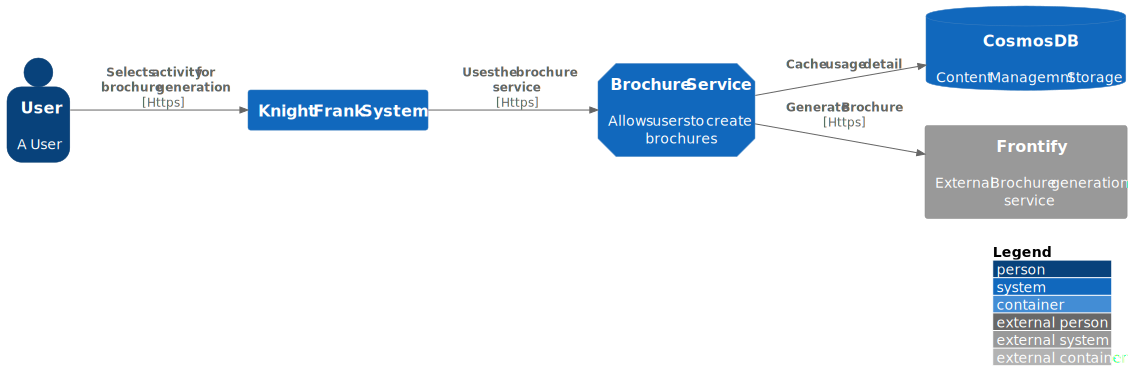
\includegraphics[keepaspectratio]{index_files/mediabag/BusinessContext.png}}

}

\caption{image}

\end{figure}%

\section{Technical Context}\label{technical-context}

\begin{figure}[H]

{\centering \pandocbounded{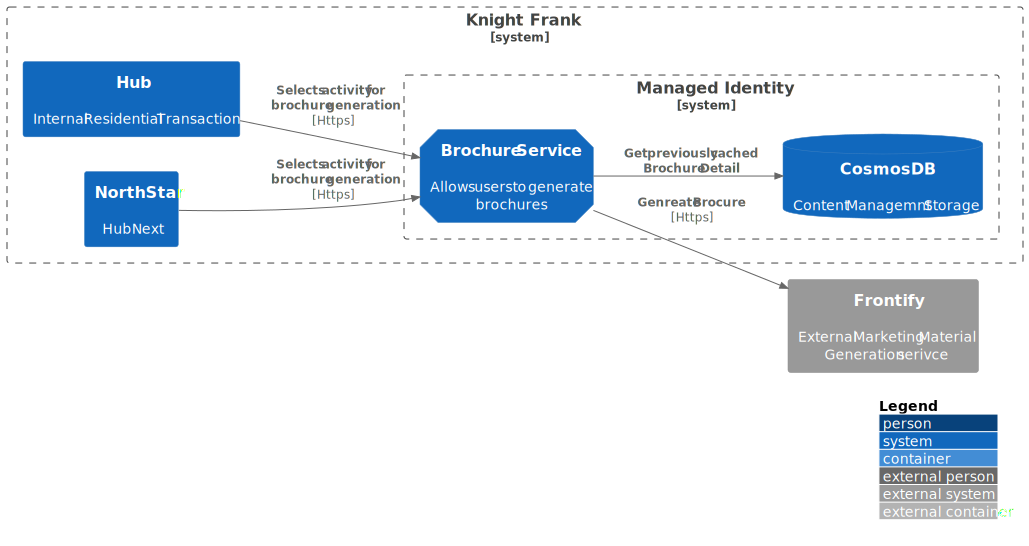
\includegraphics[keepaspectratio]{index_files/mediabag/TechnicalContext.png}}

}

\caption{image}

\end{figure}%

\begin{itemize}
\tightlist
\item
  The API runs as a microservice on our cloud platform, and will be
  accessible via a API Management interface.
\item
  The connection to the external Address provider is over HTTPS, secured
  by OAuth2.
\item
  The data passed in this application is not sensitive and doesn't need
  any encryption protocols.
\item
  Any data retuned by the external provider will be stored, by our
  document management and scanned for viruses.
\item
  A service bus interface will be available, for asynchronous queueing
  of jobs.
\item
  A http interface will be available, for ad-hoc querying of
  information.
\end{itemize}

\begin{longtable}[]{@{}ll@{}}
\toprule\noalign{}
Business Interface & Channel \\
\midrule\noalign{}
\endhead
\bottomrule\noalign{}
\endlastfoot
API for business functions & internet (https) \\
API for admin / audit & internet (https) \\
Bulk Updates & Service Bus \\
\end{longtable}

\part{Building Block View}

\begin{figure}[H]

{\centering \pandocbounded{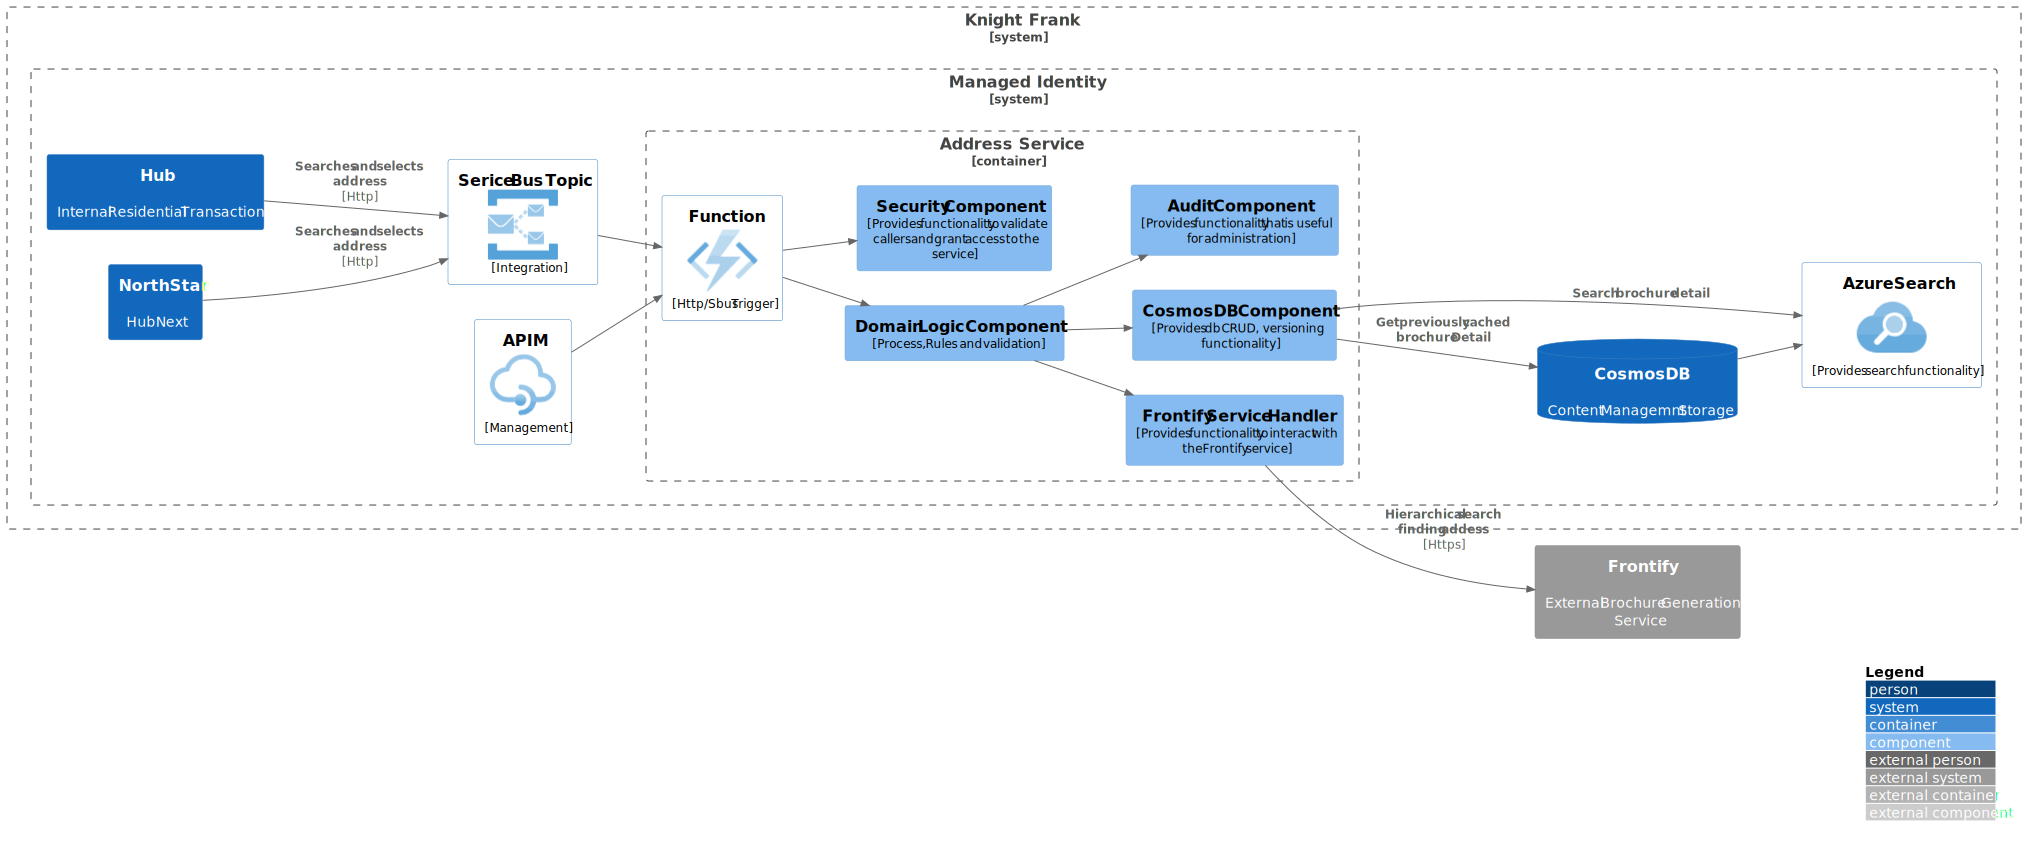
\includegraphics[keepaspectratio]{index_files/mediabag/BuildingBlockView.png}}

}

\caption{image}

\end{figure}%

This service has been designed to handle the interaction with the
Frontify brochure generation service. Based on the information supplied
the service will determine whether to use the, more automated API
service, or the more bespoke CSV file service, which requires a great
deal of user interaction.

The service will provide auditing information, which will return
information based on the quantity of requests by day/month, and by whom.

\subsection*{Contained Building Blocks}\label{contained-building-blocks}
\addcontentsline{toc}{subsection}{Contained Building Blocks}

\begin{longtable}[]{@{}
  >{\raggedright\arraybackslash}p{(\linewidth - 2\tabcolsep) * \real{0.2143}}
  >{\raggedright\arraybackslash}p{(\linewidth - 2\tabcolsep) * \real{0.7857}}@{}}
\toprule\noalign{}
\begin{minipage}[b]{\linewidth}\raggedright
\textbf{Name}
\end{minipage} & \begin{minipage}[b]{\linewidth}\raggedright
\textbf{Responsibility}
\end{minipage} \\
\midrule\noalign{}
\endhead
\bottomrule\noalign{}
\endlastfoot
Azure Function & Is the interface to all systems. provides both Restful
API and Service Bus Interfaces. \\
Security Component & Provides all Managed Identity and User
Identity/Access controls \\
Audit Component & Provides a standardised set of audit data retrieval
methods, and SOC Alert rules \\
Cosmos Db Component & Provides any abstractions or specialisations
necessary to access the Cosmos DB \\
Frontify Service Handler & Is a specific interface for the Frontify
Brochure Generation service. \\
Domain Logic Component & Provides rules and workflow to satisfy the
requirements of this service \\
\end{longtable}

\subsection*{Azure Function}\label{azure-function}
\addcontentsline{toc}{subsection}{Azure Function}

The Azure function is the external interface for the service and will
support both a RESTful API and a service bus interfaces.

The Service Bus interface is the main interface for creating brochures.

The RESTful API will follow standard REST naming conventions
e.g.~/Customers or /Customer/\{id\} to return a collection or a single
entity. The RESTful API also employ OPENAPI documentation frames
detailing the request and response models, and all return statuses.

\section*{Components}\label{components}
\addcontentsline{toc}{section}{Components}

\markright{Components}

The component libraries should be general and built so they can be
copied or included in other projects.

\subsection*{Security Component}\label{security-component}
\addcontentsline{toc}{subsection}{Security Component}

This component will validate the Managed Identity Header. This indicates
that the calling application has been authorised to use this service. If
a caller fails the Managed Identity authorisation then the method should
return a HTTP Status of 401 Unauthorised. If a user token is included,
then it should be validated with Entra Id(Active Directory) and the
returned claims inspected. Failure should result in a HTTP Status 403
Forbidden.

\subsection*{Audit Component}\label{audit-component}
\addcontentsline{toc}{subsection}{Audit Component}

Generally all audit components will implement the same API calls, this
will allow an admin application to produced consistent reporting across
the service estate. The Audit component can supply additional API
methods to return specific information that only applies to the current
service. The audit interface should be included with the service API,
and include calls to return counts based on usage by user/system.

\subsection*{Cosmos Db Component}\label{cosmos-db-component}
\addcontentsline{toc}{subsection}{Cosmos Db Component}

This component should utilise the CQRS pattern, All read requests should
be serviced by Azure Search queries. Cosmos Db should be implemented
with the NoSQL container. This component should use both the
Microsoft.Azure.Cosmos and Azure.Identity libraries. The calling client
application will be authorised by Managed Identity to access the Cosmos
DB. This component should encapsulate any company nuances which are
general to our usage of Cosmos DB, such as naming conventions or setting
configuration.

\subsection*{Frontfy Service Handler}\label{frontfy-service-handler}
\addcontentsline{toc}{subsection}{Frontfy Service Handler}

This service handler will interact with the Frontify Brochure Generation
system. All data will be passed to/from this service in a canonical
form, so internal systems are not dependant on changes to the Frontify
service.

\subsection*{Domain Logic Component}\label{domain-logic-component}
\addcontentsline{toc}{subsection}{Domain Logic Component}

The domain logic component implements the business requirements of the
service. It consists of a workflow and rules. Workflow will not contain
rules. The workflow will only ever ask questions of the rules.

\subsection*{Sequence of Interactions}\label{sequence-of-interactions}
\addcontentsline{toc}{subsection}{Sequence of Interactions}

The sequence diagram below shows the flow calls to Frontify.

The group in red is an area of discussion, as this is the manual,
bespoke, process, so the service will not be able to track changes or
completion. Meaning the incomplet objects in the datastore will keep
building, making the CSV larger and larger.

\begin{Shaded}
\begin{Highlighting}[]
\NormalTok{@startuml
}

\NormalTok{actor "Hub User" as user
}
\NormalTok{participant Hub as hub
}
\NormalTok{database HUbDb as hubdb
}
\NormalTok{queue "Service Bus" as bus
}
\NormalTok{participant Service as svc
}
\NormalTok{database CosmosDb as db
}
\NormalTok{participant "Document Manager" as dm
}
\NormalTok{participant Frontify as fmt
}
\NormalTok{actor "Frontify User" as fmtUsr
}

\NormalTok{user {-}\textgreater{} hub ++ \#gold
}
\NormalTok{  hub {-}\textgreater{} svc ++ \#gold: Get Templates
}
\NormalTok{    svc {-}\textgreater{} fmt ++ \#gold: Get Templates
}
\NormalTok{    fmt {-}{-}\textgreater{} svc {-}{-}
}
\NormalTok{  svc {-}{-}\textgreater{} hub {-}{-}
}
\NormalTok{hub {-}{-}\textgreater{} user {-}{-}: Select template
}

\NormalTok{user {-}\textgreater{} hub ++ \#gold: Create Brochure
}
\NormalTok{  hub {-}\textgreater{} bus ++ \#gold: Publish Create Brochure
}
\NormalTok{    bus {-}\textgreater{} svc ++ \#gold: Subscribe Brochure Artifacts
}
\NormalTok{    Group Create Brochure Object
}
\NormalTok{        svc {-}\textgreater{} db : Create Brochure Object
}
\NormalTok{        svc {-}\textgreater{} db : Add Text to Brochure Object
}
\NormalTok{        loop
}
\NormalTok{            svc {-}\textgreater{} fmt ++ \#gold: Load and Create Asset
}
\NormalTok{            fmt {-}{-}\textgreater{} svc {-}{-}  
}
\NormalTok{            svc {-}\textgreater{} db : Add AssetId to Brochure Object
}
\NormalTok{        end
}
\NormalTok{    End
}
\NormalTok{    Group \#pink Bespoke 
}
\NormalTok{        svc {-}\textgreater{} svc : Create CSV
}
\NormalTok{        svc {-}\textgreater{} db : Get Incomplete Brochure Objects
}
\NormalTok{        svc {-}\textgreater{} svc : Create CSV rows
}
\NormalTok{        svc {-}\textgreater{} fmt ++ \#gold: Upload CSV
}
        
\NormalTok{        fmt {-}\textgreater{} fmtUsr ++ \#gold 
}
\NormalTok{        fmtUsr {-}{-}\textgreater{} fmt {-}{-}
}
\NormalTok{        fmt {-}{-}\textgreater{} svc {-}{-}
}
\NormalTok{        ...
}
\NormalTok{        Group Brochure Completion / User
}
\NormalTok{          fmtUsr {-}\textgreater{} hub : Set Brochure Complete
}
\NormalTok{          hub {-}\textgreater{} svc : Set Brochure Complete
}
\NormalTok{          svc {-}{-}\textgreater{} hub
}
\NormalTok{        End
}

\NormalTok{    End
}
\NormalTok{    Group \#lightblue Auto
}
\NormalTok{        svc {-}\textgreater{} fmt ++ \#gold: Create Brochure Request from Brochure Object
}
\NormalTok{        fmt {-}\textgreater{} fmt : 
}
\NormalTok{        ...
}
\NormalTok{        Group Brochure Completion /  WebHook
}
\NormalTok{            fmt {-}\textgreater{} svc {-}{-}: Brochure Created
}
\NormalTok{        End     
}
\NormalTok{    End
}

\NormalTok{    svc {-}\textgreater{} fmt ++ \#gold: Get Brochure
}
\NormalTok{    fmt {-}{-}\textgreater{} svc {-}{-}
}

\NormalTok{    svc {-}\textgreater{} dm ++ \#gold: Save Brochure
}
\NormalTok{    dm {-}{-}\textgreater{} svc {-}{-}
}
\NormalTok{    svc {-}\textgreater{} db : Complete Brochure Object
}
\NormalTok{    svc {-}{-}\textgreater{} bus {-}{-}: Publish Brochure metadata
}

\NormalTok{  bus {-}\textgreater{} hub {-}{-}: Subscribe Brochure metadata
}
\NormalTok{  hub {-}\textgreater{} hubdb ++ \#gold: Save metadata
}
\NormalTok{  hubdb {-}{-}\textgreater{} hub {-}{-}: 
}
\NormalTok{hub {-}\textgreater{} user {-}{-}: Notify
}
\NormalTok{@enduml
}
\end{Highlighting}
\end{Shaded}

\subsection*{Flowchart}\label{flowchart}
\addcontentsline{toc}{subsection}{Flowchart}

\begin{Shaded}
\begin{Highlighting}[]
\NormalTok{@startuml
}

\NormalTok{start
}
\NormalTok{fork
}
\NormalTok{  : 1, Get Templates;
}
\NormalTok{  Group Hub
}
\NormalTok{    :HUB : Get Templates;
}
\NormalTok{  EndGroup
}
\NormalTok{  Group Service
}
\NormalTok{    :SVC : Get Filterd Templates and details from Frontify;
}
\NormalTok{  EndGroup
}

\NormalTok{fork again
}
\NormalTok{  : 2, Generate Brochure;
}

\NormalTok{  Group Hub
}
\NormalTok{    :Hub : Generate Text and Images;
}
\NormalTok{    :1, Get Template;     
}
    
\NormalTok{    if ( Bespoke? ) then (TRUE)
}
\NormalTok{      :Service Request : Bespoke Flag Set TRUE;
}
\NormalTok{    else (FALSE)
}
\NormalTok{      :Service Request : Bespoke Flag Set FALSE;
}
\NormalTok{    endif
}
\NormalTok{    :Service Request : Set TemplateId;
}
\NormalTok{    :Service Request : Map Text and Images\textbackslash{}n into Svc Request with Template Keys;
}
\NormalTok{  Endgroup
}

\NormalTok{  Group Service Bus
}
\NormalTok{    :Pass Service Request;
}
\NormalTok{  Endgroup
}
\NormalTok{  Group Service
}
\NormalTok{    Group Create CosmosDB Brochure Object
}
\NormalTok{    :SVC : Create a Brochure Object in Datastore;
}
\NormalTok{    :SVC : Store Text in Brochure Object;
}

\NormalTok{      Group Asset Upload
}
\NormalTok{        repeat
}
\NormalTok{            :Upload Image to Frontify;
}
\NormalTok{            :Save AssetId in Brochure Object;
}
\NormalTok{        repeat while (More images to upload?) is (yes) not (no)
}
\NormalTok{      EndGroup
}
\NormalTok{    EndGroup
}

\NormalTok{    if (Generate Bespoke Brochure?) then (TRUE)
}
\NormalTok{      Group Generate CSV
}
\NormalTok{        :Get All incomplete BESPOKE Brochures from Datastore;
}
\NormalTok{        :Create CSV;
}
\NormalTok{        repeat
}
\NormalTok{          :Get Brochure Object;
}
\NormalTok{          :CSV: New Row;
}
\NormalTok{          :CSV: Add Texts to matching column heading;
}
\NormalTok{          :CSV: Add AssetIds to matching column heading;
}
\NormalTok{        repeat while (More Brochure Objects?) is (yes) not (no)
}

\NormalTok{        :Upload CSV;
}
\NormalTok{        :User : Generate Brochure;
}
\NormalTok{        :3, Complete Brochure; 
}
\NormalTok{      EndGroup
}

\NormalTok{    else (FALSE)
}
\NormalTok{      Group Auto Generate
}
\NormalTok{        :Using Current Brochure Object;
}
\NormalTok{        :ExportCreative and Associate Assets and Template;
}
\NormalTok{        :Generate Brochure {-} Returns Brochure Id;
}
\NormalTok{      EndGroup
}
\NormalTok{    Group CleanUp
}
\NormalTok{      :Check Brochure Status;
}
\NormalTok{      :Get Brochure;
}
\NormalTok{      :Store Brochure;
}
\NormalTok{      :Complete Datastore Brochure Object;
}
\NormalTok{    EndGroup
}

\NormalTok{    Group Service Bus
}
\NormalTok{      :Return Brochure Metadata;
}
\NormalTok{    Endgroup
}
\NormalTok{    endif
}
\NormalTok{  EndGroup
}

\NormalTok{fork again
}
\NormalTok{  : 3, Complete Brochure;
}
\NormalTok{  Group Hub
}
\NormalTok{    :HUB : Complete Brochure;
}
\NormalTok{  EndGroup
}
\NormalTok{  Group Service
}
\NormalTok{    :SVC : Mark datastore Brochure Object Complete;
}
\NormalTok{  EndGroup
}
\NormalTok{endfork
}
\NormalTok{stop
}

\NormalTok{@enduml
}
\end{Highlighting}
\end{Shaded}

\subsection*{Component Detail}\label{component-detail}
\addcontentsline{toc}{subsection}{Component Detail}

\begin{enumerate}
\def\labelenumi{\arabic{enumi}.}
\tightlist
\item
  Azure Function Detail
\item
  Security Component
\item
  Service Component
\item
  Domain Logic Component
\item
  Cosmos DB Component
\end{enumerate}

\chapter{Azure Function Detail}\label{azure-function-detail}

{[}{[}TOC{]}{]}

\subsection{Azure Function}\label{azure-function-1}

\pandocbounded{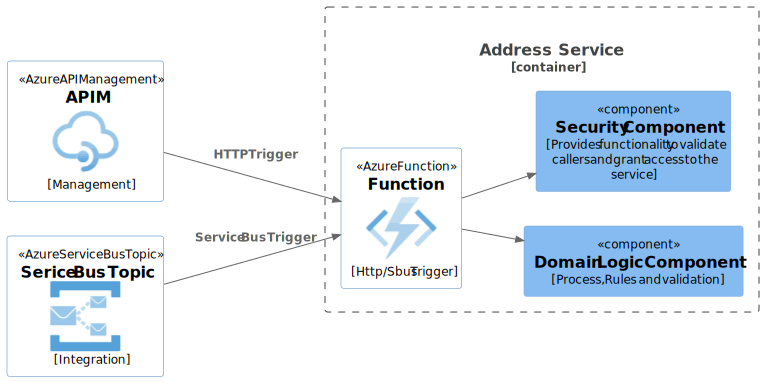
\includegraphics[keepaspectratio]{index_files/mediabag/AzureFunction.png}}

\subsubsection{RESTFul API}\label{restful-api}

\textbf{Brochure}

\textbf{Get Templates}

\begin{itemize}
\tightlist
\item
  Returns a list of templates
\item
  Flow
\end{itemize}

\begin{Shaded}
\begin{Highlighting}[]
\NormalTok{@startuml
}
\NormalTok{Group Service
}
\NormalTok{  start
}
\NormalTok{    :Get Template request;
}
\NormalTok{    :Get Templates from Frontify;
}
\NormalTok{    :Filter Templates by Auto Generation indicator;
}
\NormalTok{    :Return Template List;
}
\NormalTok{  stop
}
\NormalTok{EndGroup
}

\NormalTok{@enduml}
\end{Highlighting}
\end{Shaded}

\begin{itemize}
\item
  URL : /Templates
\item
  Parameters : None
\item
  HTTP Method : GET
\item
  Request Body : None
\item
  Response Body
\item
  HTTP Errors

  \begin{longtable}[]{@{}ll@{}}
  \toprule\noalign{}
  Error & Meaning \\
  \midrule\noalign{}
  \endhead
  \bottomrule\noalign{}
  \endlastfoot
  2xx & OK(Success) \\
  4xx & User Failure \\
  5xx & System Failure \\
  \end{longtable}
\item
  Response Body
\end{itemize}

\begin{Shaded}
\begin{Highlighting}[]
\NormalTok{@startjson
}
\NormalTok{\{
}
\NormalTok{    "Templates": [
}
\NormalTok{        \{
}
\NormalTok{            "TemplateId": "string",
}
\NormalTok{            "Name": "string",
}
\NormalTok{            "Description": "string",
}
\NormalTok{            "Details": [
}
\NormalTok{                \{
}
\NormalTok{                    "Key": "string",
}
\NormalTok{                    "Type": "Text/Image"
}
\NormalTok{                \}
}
\NormalTok{            ]              
}
\NormalTok{        \}
}
\NormalTok{    ]
}
\NormalTok{\}
}
\NormalTok{@endjson
}
\end{Highlighting}
\end{Shaded}

\textbf{N.B. The Details array forms the Details array of the brochure
request.}

\textbf{Complete Brochure}

\begin{Shaded}
\begin{Highlighting}[]
\NormalTok{@startuml
}
\NormalTok{  : 3, Complete Brochure;
}
\NormalTok{  Group Hub
}
\NormalTok{    :HUB : Complete Brochure;
}
\NormalTok{  EndGroup
}
\NormalTok{  Group Service
}
\NormalTok{    :SVC : Mark datastore Brochure Object Complete;
}
\NormalTok{  EndGroup
}
\NormalTok{@enduml}
\end{Highlighting}
\end{Shaded}

\begin{longtable}[]{@{}lll@{}}
\toprule\noalign{}
\endhead
\bottomrule\noalign{}
\endlastfoot
URL & /CompleteBrochure & \\
Parameters & & \\
& ExternalId & Id of the calling system \\
HTTP Method & GET & \\
Request Body & None & \\
Response Body & None & \\
HTTP Errors & 2xx & OK(Success) \\
& 4xx & User Failure \\
& 5xx & System Failure \\
\end{longtable}

\textbf{Audit}

\textbf{Get By Source App}

\begin{itemize}
\tightlist
\item
  Returns the count of requests made by source Application
\item
  URL \textbf{/SourceApp/}
\item
  HTTP Method \textbf{GET}
\item
  Parameters

  \begin{itemize}
  \tightlist
  \item
    \textbf{None} - returns an list of source apps and there counts
  \item
    \textbf{SourceApp} - returns the count made by the passed SourceApp
  \end{itemize}
\item
  Request Body \textbf{None}
\item
  Response Body
\end{itemize}

\begin{Shaded}
\begin{Highlighting}[]
\NormalTok{@startjson
}
\NormalTok{[
}
\NormalTok{    \{
}
\NormalTok{        "SourceApp": "string",
}
\NormalTok{        "Count": "string\textless{}number\textgreater{}"
}
\NormalTok{    \}
}
\NormalTok{]
}
\NormalTok{@endjson}
\end{Highlighting}
\end{Shaded}

\begin{itemize}
\item
  HTTP Errors

  \begin{longtable}[]{@{}ll@{}}
  \toprule\noalign{}
  Error & Meaning \\
  \midrule\noalign{}
  \endhead
  \bottomrule\noalign{}
  \endlastfoot
  2xx & OK(Success) \\
  4xx & User Failure \\
  5xx & System Failure \\
  \end{longtable}
\end{itemize}

\textbf{Get By User}

\begin{itemize}
\tightlist
\item
  Returns the count of requests made by User
\item
  URL \textbf{/User/ param / (optional) Detail}
\item
  HTTP Method \textbf{GET}
\item
  Parameters

  \begin{itemize}
  \tightlist
  \item
    \textbf{None} - returns an list of User and their counts

    \begin{itemize}
    \tightlist
    \item
      Cannot add detail
    \end{itemize}
  \item
    Id** - returns the count made by the passed User
  \item
    \textbf{Login} - returns the count made by the passed User
  \item
    \textbf{Email} - returns the count made by the passed User
  \end{itemize}
\item
  Request Body \textbf{None}
\item
  Response Body

  \begin{itemize}
  \tightlist
  \item
    Count Response
  \end{itemize}
\end{itemize}

\begin{Shaded}
\begin{Highlighting}[]
\NormalTok{@startjson
}
\NormalTok{\{
}
\NormalTok{    "User": \{
}
\NormalTok{        "id" : "string\textless{}uuid\textgreater{}",
}
\NormalTok{        "login": "string",
}
\NormalTok{        "name": "string",
}
\NormalTok{        "email": "string"
}
\NormalTok{    \},
}
\NormalTok{    "Count": "string\textless{}number\textgreater{}"
}
\NormalTok{\}
}
\NormalTok{@endjson
}

\end{Highlighting}
\end{Shaded}

\begin{itemize}
\tightlist
\item
  Detail response
\end{itemize}

\begin{Shaded}
\begin{Highlighting}[]
\NormalTok{@startjson
}
\NormalTok{\{
}
\NormalTok{    "User": \{
}
\NormalTok{        "id" : "string\textless{}uuid\textgreater{}",
}
\NormalTok{        "login": "string",
}
\NormalTok{        "name": "string",
}
\NormalTok{        "email": "string"
}
\NormalTok{    \},
}
\NormalTok{    "Count": "string\textless{}number\textgreater{}",
}
\NormalTok{    "Requests" : [
}
\NormalTok{        \{
}
\NormalTok{            "Id": "string",
}
\NormalTok{            "When" : "string\textless{}DateTime\textgreater{}",
}
\NormalTok{            "SourceApp": "string"
}
\NormalTok{        \}
}
\NormalTok{    ]
}
\NormalTok{\}
}
\NormalTok{@endjson
}
\end{Highlighting}
\end{Shaded}

\begin{itemize}
\item
  HTTP Errors

  \begin{longtable}[]{@{}ll@{}}
  \toprule\noalign{}
  Error & Meaning \\
  \midrule\noalign{}
  \endhead
  \bottomrule\noalign{}
  \endlastfoot
  2xx & OK(Success) \\
  4xx & User Failure \\
  5xx & System Failure \\
  \end{longtable}
\end{itemize}

\textbf{Get By Impersonating}

\begin{itemize}
\tightlist
\item
  Returns the count of requests made by Impersonating
\item
  URL \textbf{/Impersonating/ param / (optional) Detail}
\item
  HTTP Method \textbf{GET}
\item
  Parameters

  \begin{itemize}
  \tightlist
  \item
    \textbf{None} - returns an list of Impersonating and their counts

    \begin{itemize}
    \tightlist
    \item
      Cannot add detail
    \end{itemize}
  \item
    \textbf{Id} - returns the count made by the passed Impersonating
  \item
    \textbf{Login} - returns the count made by the passed Impersonating
  \item
    \textbf{Email} - returns the count made by the passed Impersonating
  \end{itemize}
\item
  Request Body \textbf{None}
\item
  Response Body

  \begin{itemize}
  \tightlist
  \item
    Count Response
  \end{itemize}
\end{itemize}

\begin{Shaded}
\begin{Highlighting}[]
\NormalTok{@startjson
}
\NormalTok{\{
}
\NormalTok{    "Impersonating": \{
}
\NormalTok{        "id" : "string\textless{}uuid\textgreater{}",
}
\NormalTok{        "login": "string",
}
\NormalTok{        "name": "string",
}
\NormalTok{        "email": "string"
}
\NormalTok{    \},
}
\NormalTok{    "Count": "string\textless{}number\textgreater{}"
}
\NormalTok{\}
}
\NormalTok{@endjson
}
\end{Highlighting}
\end{Shaded}

\begin{itemize}
\tightlist
\item
  Detail response
\end{itemize}

\begin{Shaded}
\begin{Highlighting}[]
\NormalTok{@startjson
}
\NormalTok{\{
}
\NormalTok{    "Impersonating": \{
}
\NormalTok{        "id" : "string\textless{}uuid\textgreater{}",
}
\NormalTok{        "login": "string",
}
\NormalTok{        "name": "string",
}
\NormalTok{        "email": "string"
}
\NormalTok{    \},
}
\NormalTok{    "Count": "string\textless{}number\textgreater{}",
}
\NormalTok{    "Requests" : [
}
\NormalTok{        \{
}
\NormalTok{            "Id": "string",
}
\NormalTok{            "When" : "string\textless{}DateTime\textgreater{}",
}
\NormalTok{            "Sourced": "Ext/int"
}
\NormalTok{        \}
}
\NormalTok{    ]
}
\NormalTok{\}
}
\NormalTok{@endjson}
\end{Highlighting}
\end{Shaded}

\begin{itemize}
\item
  HTTP Errors

  \begin{longtable}[]{@{}ll@{}}
  \toprule\noalign{}
  Error & Meaning \\
  \midrule\noalign{}
  \endhead
  \bottomrule\noalign{}
  \endlastfoot
  2xx & OK(Success) \\
  4xx & User Failure \\
  5xx & System Failure \\
  \end{longtable}
\end{itemize}

\textbf{Get By Host}

\begin{itemize}
\item
  Returns the count of requests made by Host
\item
  URL \textbf{/Host/ param / (optional) Detail}
\item
  HTTP Method \textbf{GET}
\item
  Parameters

  \begin{longtable}[]{@{}lll@{}}
  \toprule\noalign{}
  Parameter & Description & Detail \\
  \midrule\noalign{}
  \endhead
  \bottomrule\noalign{}
  \endlastfoot
  None & Returns an list of Host and their count & \\
  \textbf{IpAddress} & Returns the count made by the passed Host &
  Optional \\
  \textbf{hostName} & Returns the count made by the passed Host &
  Optional \\
  \end{longtable}
\item
  Request Body \textbf{None}
\item
  Errors

  \begin{longtable}[]{@{}ll@{}}
  \toprule\noalign{}
  Http Status Code & Meaning \\
  \midrule\noalign{}
  \endhead
  \bottomrule\noalign{}
  \endlastfoot
  200(OK) & Success \\
  4xx & User request error \\
  5xx & System Error \\
  \end{longtable}
\item
  Response Body

  \begin{longtable}[]{@{}
    >{\raggedright\arraybackslash}p{(\linewidth - 4\tabcolsep) * \real{0.2289}}
    >{\raggedright\arraybackslash}p{(\linewidth - 4\tabcolsep) * \real{0.2169}}
    >{\raggedright\arraybackslash}p{(\linewidth - 4\tabcolsep) * \real{0.5542}}@{}}
  \toprule\noalign{}
  \begin{minipage}[b]{\linewidth}\raggedright
  Path
  \end{minipage} & \begin{minipage}[b]{\linewidth}\raggedright
  Type
  \end{minipage} & \begin{minipage}[b]{\linewidth}\raggedright
  Description
  \end{minipage} \\
  \midrule\noalign{}
  \endhead
  \bottomrule\noalign{}
  \endlastfoot
  Host.IpAddress & string\textless ipAddress\textgreater{} & The Ip
  Address of the requesting host \\
  Host.hostName & string & The name of the requesting host \\
  Count & string\textless number\textgreater{} & The total number of
  requests made \\
  Requests & Array & \\
  Requests{[}{]}.Id & string\textless uuid\textgreater{} & Id of the
  request \\
  Requests{[}{]}.When & string\textless DateTime\textgreater{} & When
  the request was made \\
  Requests{[}{]}.Sourced & string & Ext/Int, was it a external or
  internal request \\
  \end{longtable}

  \begin{itemize}
  \tightlist
  \item
    Count Response
  \end{itemize}
\end{itemize}

\begin{Shaded}
\begin{Highlighting}[]
\NormalTok{@startjson
}
\NormalTok{\{
}
\NormalTok{    "Host":\{
}
\NormalTok{        "ipAddress":"string\textless{}ipv4\textgreater{}",
}
\NormalTok{        "hostName":"string\textless{}hostname\textgreater{}"
}
\NormalTok{    \},
}
\NormalTok{    "Count": "string\textless{}number\textgreater{}"
}
\NormalTok{\}
}
\NormalTok{@endjson}
\end{Highlighting}
\end{Shaded}

\begin{verbatim}
*   Detail response
\end{verbatim}

\begin{Shaded}
\begin{Highlighting}[]
\NormalTok{@startjson
}
\NormalTok{\{
}
\NormalTok{    "Host":\{
}
\NormalTok{        "ipAddress":"string\textless{}ipv4\textgreater{}",
}
\NormalTok{        "hostName":"string\textless{}hostname\textgreater{}"
}
\NormalTok{    \},
}
\NormalTok{    "Count": "string\textless{}number\textgreater{}",
}
\NormalTok{    "Requests" : [
}
\NormalTok{        \{
}
\NormalTok{            "Id": "string",
}
\NormalTok{            "When" : "string\textless{}DateTime\textgreater{}",
}
\NormalTok{            "Sourced": "Ext/int"
}
\NormalTok{        \}
}
\NormalTok{    ]
}
\NormalTok{\}
}
\NormalTok{@endjson}
\end{Highlighting}
\end{Shaded}

\subsubsection{Service Bus}\label{service-bus}

\textbf{Request}

\begin{Shaded}
\begin{Highlighting}[]
\NormalTok{@startjson
}
\NormalTok{\{
}
\NormalTok{    "Audit": \{
}
\NormalTok{        "sourceApp": "string",
}
\NormalTok{        "user": \{
}
\NormalTok{            "id" : "string\textless{}uuid\textgreater{}",
}
\NormalTok{            "login": "string",
}
\NormalTok{            "name": "string",
}
\NormalTok{            "email": "string"
}
\NormalTok{        \},
}
\NormalTok{        "impersonating": \{
}
\NormalTok{            "id" : "string\textless{}uuid\textgreater{}",
}
\NormalTok{            "login": "string",
}
\NormalTok{            "name": "string",
}
\NormalTok{            "email": "string"
}
\NormalTok{        \},
}
\NormalTok{        "host":\{
}
\NormalTok{            "ipAddress":"string\textless{}ipv4\textgreater{}",
}
\NormalTok{            "hostName":"string\textless{}hostname\textgreater{}"
}
\NormalTok{        \},
}
\NormalTok{        "timestamp": "string\textless{}datetime\textgreater{}"
}
\NormalTok{    \},
}
\NormalTok{    "Request" : \{
}
\NormalTok{        "Id": "string\textless{}GUID\textgreater{}",
}
\NormalTok{        "Custom" : "string\textless{}boolean\textgreater{}",
}
\NormalTok{        "TemplateId": "string\textless{}FrontifyId\textgreater{}",
}
\NormalTok{        "Brochure": [
}
\NormalTok{            \{ 
}
\NormalTok{              "Key": "string",
}
\NormalTok{              "Type": "string",
}
\NormalTok{              "Value": "string"
}
\NormalTok{            \}
}
\NormalTok{        ]
}
\NormalTok{    \}
}
\NormalTok{\}
}

\NormalTok{@endjson}
\end{Highlighting}
\end{Shaded}

\begin{longtable}[]{@{}
  >{\raggedright\arraybackslash}p{(\linewidth - 6\tabcolsep) * \real{0.1190}}
  >{\raggedright\arraybackslash}p{(\linewidth - 6\tabcolsep) * \real{0.0357}}
  >{\raggedright\arraybackslash}p{(\linewidth - 6\tabcolsep) * \real{0.0833}}
  >{\raggedright\arraybackslash}p{(\linewidth - 6\tabcolsep) * \real{0.7619}}@{}}
\toprule\noalign{}
\begin{minipage}[b]{\linewidth}\raggedright
Column
\end{minipage} & \begin{minipage}[b]{\linewidth}\raggedright
M/O
\end{minipage} & \begin{minipage}[b]{\linewidth}\raggedright
Type
\end{minipage} & \begin{minipage}[b]{\linewidth}\raggedright
Description
\end{minipage} \\
\midrule\noalign{}
\endhead
\bottomrule\noalign{}
\endlastfoot
Id & M & Guid & Unique identifier \\
Custom & M & Boolean & Generate a custom brochure (manual) \\
TemplateId & O & string & Id of the template stored in the Frontify
system \\
Brochure & M & & Array of Key/Value pairs which make up the body of the
brochure. \\
& & & - If the Type is TEXT then value is normal text \\
& & & - If the Type is IMAGE then value is could be :- \\
& & & - GUID then get the image from the DM \\
& & & - Base64 string, it is the image \\
& & & - path then get the image from the OG hub storage (maybe) \\
Audit & M & & Common Audit information supplied to all services \\
\end{longtable}

\textbf{Response}

\begin{Shaded}
\begin{Highlighting}[]
\NormalTok{@startjson
}
\NormalTok{\{
}
\NormalTok{    "Audit": \{
}
\NormalTok{        "sourceApp": "string",
}
\NormalTok{        "user": \{
}
\NormalTok{            "id" : "string\textless{}uuid\textgreater{}",
}
\NormalTok{            "login": "string",
}
\NormalTok{            "name": "string",
}
\NormalTok{            "email": "string"
}
\NormalTok{        \},
}
\NormalTok{        "impersonating": \{
}
\NormalTok{            "id" : "string\textless{}uuid\textgreater{}",
}
\NormalTok{            "login": "string",
}
\NormalTok{            "name": "string",
}
\NormalTok{            "email": "string"
}
\NormalTok{        \},
}
\NormalTok{        "host":\{
}
\NormalTok{            "ipAddress":"string\textless{}ipv4\textgreater{}",
}
\NormalTok{            "hostName":"string\textless{}hostname\textgreater{}"
}
\NormalTok{        \},
}
\NormalTok{        "timestamp": "string\textless{}datetime\textgreater{}"
}
\NormalTok{    \},
}
\NormalTok{    "Request" : \{
}
\NormalTok{        "Id": "string\textless{}GUID\textgreater{}",
}
\NormalTok{        "Custom" : "string\textless{}boolean\textgreater{}",
}
\NormalTok{        "TemplateId": "string\textless{}FrontifyId\textgreater{}",
}
\NormalTok{        "Brochure": [
}
\NormalTok{            \{ 
}
\NormalTok{              "Key": "string",
}
\NormalTok{              "Type": "string",
}
\NormalTok{              "Value": "string"
}
\NormalTok{            \}
}
\NormalTok{        ]
}
\NormalTok{    \},
}
\NormalTok{    "Response": \{
}
\NormalTok{      "Brochure" : \{
}
\NormalTok{        "DocManagerId": "string\textless{}GUID\textgreater{}",
}
\NormalTok{        "URL": "string\textless{}URL\textgreater{}"
}
\NormalTok{      \}
}
\NormalTok{    \},
}
\NormalTok{    "Error" : [
}
\NormalTok{      \{
}
\NormalTok{        "Desctiption" : "String"
}
\NormalTok{      \}
}
\NormalTok{    ]    
}
\NormalTok{\}
}
\NormalTok{@endjson
}
\end{Highlighting}
\end{Shaded}

\chapter{Cosmos Db Component}\label{cosmos-db-component-1}

A NoSql Cosmos DB container should be used as this service is similar in
operation to other services, and also due to the variable length of
Brochure array.

\section{Containers}\label{containers}

\begin{Shaded}
\begin{Highlighting}[]
\NormalTok{@startjson
}
\NormalTok{\{
}
\NormalTok{    "Id" : "string",
}
\NormalTok{    "Audit": \{
}
\NormalTok{        "sourceApp": "string",
}
\NormalTok{        "user": \{
}
\NormalTok{            "id" : "string\textless{}uuid\textgreater{}",
}
\NormalTok{            "login": "string",
}
\NormalTok{            "name": "string",
}
\NormalTok{            "email": "string"
}
\NormalTok{        \},
}
\NormalTok{        "impersonating": \{
}
\NormalTok{            "id" : "string\textless{}uuid\textgreater{}",
}
\NormalTok{            "login": "string",
}
\NormalTok{            "name": "string",
}
\NormalTok{            "email": "string"
}
\NormalTok{        \},
}
\NormalTok{        "host":\{
}
\NormalTok{            "ipAddress":"string\textless{}ipv4\textgreater{}",
}
\NormalTok{            "hostName":"string\textless{}hostname\textgreater{}"
}
\NormalTok{        \},
}
\NormalTok{        "timestamp": "string\textless{}datetime\textgreater{}"
}
\NormalTok{    \},
}
\NormalTok{    "Request" : \{
}
\NormalTok{        "ExternalId": "string\textless{}guid\textgreater{}",
}
\NormalTok{        "Bespoke" : "string\textless{}boolean\textgreater{}",
}
\NormalTok{        "TemplateId": "string\textless{}FrontifyId\textgreater{}",
}
\NormalTok{        "Brochure": [
}
\NormalTok{            \{ 
}
\NormalTok{              "Key": "string",
}
\NormalTok{              "Type": "string",
}
\NormalTok{              "Value": "string"
}
\NormalTok{            \}
}
\NormalTok{        ]
}
\NormalTok{    \},
}
\NormalTok{    "Error" : [
}
\NormalTok{      \{
}
\NormalTok{        "Desctiption" : "String"
}
\NormalTok{      \}
}
\NormalTok{    ]    
}
\NormalTok{\}
}
\NormalTok{@enduml
}
\end{Highlighting}
\end{Shaded}

\chapter{Domain Logic Component}\label{domain-logic-component-1}

The domain logic will handle requests from both Service Bus and Ad-hoc
via a RESTful API interface. Audit enquires will be routed to the audit
component.

\section{Flowchart}\label{flowchart-1}

\begin{Shaded}
\begin{Highlighting}[]
\NormalTok{@startuml
}

\NormalTok{start
}
\NormalTok{fork
}
\NormalTok{  : 1, Get Templates;
}
\NormalTok{  Group Hub
}
\NormalTok{    :HUB : Get Templates;
}
\NormalTok{  EndGroup
}
\NormalTok{  Group Service
}
\NormalTok{    :SVC : Get Filterd Templates and details from Frontify;
}
\NormalTok{  EndGroup
}

\NormalTok{fork again
}
\NormalTok{  : 2, Generate Brochure;
}

\NormalTok{  Group Hub
}
\NormalTok{    :Hub : Generate Text and Images;
}
\NormalTok{    :1, Get Template;     
}
    
\NormalTok{    if ( Bespoke? ) then (TRUE)
}
\NormalTok{      :Service Request : Bespoke Flag Set TRUE;
}
\NormalTok{    else (FALSE)
}
\NormalTok{      :Service Request : Bespoke Flag Set FALSE;
}
\NormalTok{    endif
}
\NormalTok{    :Service Request : Set TemplateId;
}
\NormalTok{    :Service Request : Map Text and Images\textbackslash{}n into Svc Request with Template Keys;
}
\NormalTok{  Endgroup
}

\NormalTok{  Group Service Bus
}
\NormalTok{    :Pass Service Request;
}
\NormalTok{  Endgroup
}
\NormalTok{  Group Service
}
\NormalTok{    Group Create CosmosDB Brochure Object
}
\NormalTok{    :SVC : Create a Brochure Object in Datastore;
}
\NormalTok{    :SVC : Store Text in Brochure Object;
}

\NormalTok{      Group Asset Upload
}
\NormalTok{        repeat
}
\NormalTok{            :Upload Image to Frontify;
}
\NormalTok{            :Save AssetId in Brochure Object;
}
\NormalTok{        repeat while (More images to upload?) is (yes) not (no)
}
\NormalTok{      EndGroup
}
\NormalTok{    EndGroup
}

\NormalTok{    if (Generate Bespoke Brochure?) then (TRUE)
}
\NormalTok{      Group Generate CSV
}
\NormalTok{        :Get All incomplete BESPOKE Brochures from Datastore;
}
\NormalTok{        :Create CSV;
}
\NormalTok{        repeat
}
\NormalTok{          :Get Brochure Object;
}
\NormalTok{          :CSV: New Row;
}
\NormalTok{          :CSV: Add Texts to matching column heading;
}
\NormalTok{          :CSV: Add AssetIds to matching column heading;
}
\NormalTok{        repeat while (More Brochure Objects?) is (yes) not (no)
}

\NormalTok{        :Upload CSV;
}
\NormalTok{        :User : Generate Brochure;
}
\NormalTok{        :3, Complete Brochure; 
}
\NormalTok{      EndGroup
}

\NormalTok{    else (FALSE)
}
\NormalTok{      Group Auto Generate
}
\NormalTok{        :Using Current Brochure Object;
}
\NormalTok{        :ExportCreative and Associate Assets and Template;
}
\NormalTok{        :Generate Brochure {-} Returns Brochure Id;
}
\NormalTok{      EndGroup
}
\NormalTok{    Group CleanUp
}
\NormalTok{      :Check Brochure Status;
}
\NormalTok{      :Get Brochure;
}
\NormalTok{      :Store Brochure;
}
\NormalTok{      :Complete Datastore Brochure Object;
}
\NormalTok{    EndGroup
}

\NormalTok{    Group Service Bus
}
\NormalTok{      :Return Brochure Metadata;
}
\NormalTok{    Endgroup
}
\NormalTok{    endif
}
\NormalTok{  EndGroup
}

\NormalTok{fork again
}
\NormalTok{  : 3, Complete Brochure;
}
\NormalTok{  Group Hub
}
\NormalTok{    :HUB : Complete Brochure;
}
\NormalTok{  EndGroup
}
\NormalTok{  Group Service
}
\NormalTok{    :SVC : Mark datastore Brochure Object Complete;
}
\NormalTok{  EndGroup
}
\NormalTok{endfork
}
\NormalTok{stop
}

\NormalTok{@enduml
}
\end{Highlighting}
\end{Shaded}

\section{Schemas and Maps}\label{schemas-and-maps}

This service takes a standard integration approach to mapping internal
and external data structures, this design breaks dependencies so that
the external interface may change without affecting internal systems.

Objects received from interfaces should follow a standard VETER
integration pattern (Validate, Extract, Transform, Enrich, Route)

\begin{itemize}
\tightlist
\item
  Validate

  \begin{itemize}
  \tightlist
  \item
    Objects should be validated and a default rules set should be
    applied to validate the object.
  \end{itemize}
\item
  Extract

  \begin{itemize}
  \tightlist
  \item
    Extract specific information from the message, such as audit etc.
  \end{itemize}
\item
  TransForm

  \begin{itemize}
  \tightlist
  \item
    The Message should be transformed into the next type in the process.
  \end{itemize}
\item
  Enrich

  \begin{itemize}
  \tightlist
  \item
    Adds additional data to the message, often from external sources
  \end{itemize}
\item
  Route

  \begin{itemize}
  \tightlist
  \item
    Directs the processed message to the appropriate destination based
    on certain criteria.
  \end{itemize}
\end{itemize}

\begin{Shaded}
\begin{Highlighting}[]
\NormalTok{@startuml
}
\NormalTok{!includeurl https://raw.githubusercontent.com/plantuml{-}stdlib/EIP{-}PlantUML/main/dist/EIP{-}PlantUML.puml
}
\NormalTok{{-}{-} !include not found: \textless{}C4/C4\_Component\textgreater{}
}
\NormalTok{AddElementTag("storage", $shape=RoundedBoxShape(), $fontColor="white")
}
\NormalTok{LAYOUT\_TOP\_DOWN()
}

\NormalTok{MessageEndpoint( svc, "Service Request" )
}
\NormalTok{Message( req, "Request")
}
\NormalTok{Message( loq, "Frontify Request")
}
\NormalTok{MessageEndpoint(frontify, "Frontify Request" )
}

\NormalTok{System\_Boundary(c1, "Domain") \{
}
\NormalTok{    SelectiveConsumer(reqval, "Validation")
}
\NormalTok{    MessageTranslator( req2con, "Request to Canonical")
}
\NormalTok{    MessageTranslator( con2loq, "Canonical to Frontify")
}
\NormalTok{    Message( con, "Canonical")
}
\NormalTok{    Message( conr, "Canonical")
}
\NormalTok{    MessageTranslator( loqr2conr, "Frontify Response to Canonical")
}
\NormalTok{    SelectiveConsumer(resval, "Validation")
}

\NormalTok{    con {-}{-} conr
}
\NormalTok{\}
}
\NormalTok{SystemDb(cosmos, "CosmosDB", "Content Managemnt Storage", $tags = "storage")
}
\NormalTok{conr {-}{-}\textgreater{} cosmos
}

\NormalTok{MessageEndpoint( svcr, "Service Response" )
}
\NormalTok{Message( res, "Response")
}
\NormalTok{Message( loqr, "Frontify Response")
}
\NormalTok{MessageEndpoint(frontifyr, "Frontify Response" )
}

\NormalTok{svc {-}\textgreater{} req
}
\NormalTok{req {-}\textgreater{} reqval
}
\NormalTok{reqval {-}\textgreater{} req2con
}
\NormalTok{req2con {-}\textgreater{} con
}
\NormalTok{con {-}\textgreater{} con2loq
}
\NormalTok{con2loq {-}\textgreater{} loq
}
\NormalTok{loq {-}\textgreater{} frontify
}

\NormalTok{req {-}[hidden]{-}\textgreater{} res
}

\NormalTok{svcr \textless{}{-} res
}
\NormalTok{res \textless{}{-} conr
}
\NormalTok{conr \textless{}{-} loqr2conr
}
\NormalTok{loqr2conr \textless{}{-} resval
}
\NormalTok{resval \textless{}{-} loqr
}
\NormalTok{loqr \textless{}{-} frontifyr
}

\NormalTok{@enduml
}
\end{Highlighting}
\end{Shaded}

\section{Brochure Generation}\label{brochure-generation}

\subsection{Request Schema}\label{request-schema}

\begin{Shaded}
\begin{Highlighting}[]
\NormalTok{@startjson
}
\NormalTok{\{
}
\NormalTok{    "Audit": \{
}
\NormalTok{        "sourceApp": "string",
}
\NormalTok{        "user": \{
}
\NormalTok{            "id" : "string\textless{}uuid\textgreater{}",
}
\NormalTok{            "login": "string",
}
\NormalTok{            "name": "string",
}
\NormalTok{            "email": "string"
}
\NormalTok{        \},
}
\NormalTok{        "impersonating": \{
}
\NormalTok{            "id" : "string\textless{}uuid\textgreater{}",
}
\NormalTok{            "login": "string",
}
\NormalTok{            "name": "string",
}
\NormalTok{            "email": "string"
}
\NormalTok{        \},
}
\NormalTok{        "host":\{
}
\NormalTok{            "ipAddress":"string\textless{}ipv4\textgreater{}",
}
\NormalTok{            "hostName":"string\textless{}hostname\textgreater{}"
}
\NormalTok{        \},
}
\NormalTok{        "timestamp": "string\textless{}datetime\textgreater{}"
}
\NormalTok{    \},
}
\NormalTok{    "Request" : \{
}
\NormalTok{        "Id": "string\textless{}GUID\textgreater{}",
}
\NormalTok{        "Custom" : "string\textless{}boolean\textgreater{}",
}
\NormalTok{        "TemplateId": "string\textless{}FrontifyId\textgreater{}",
}
\NormalTok{        "Brochure": [
}
\NormalTok{            \{ 
}
\NormalTok{              "Key": "string",
}
\NormalTok{              "Type": "string",
}
\NormalTok{              "Value": "string"
}
\NormalTok{            \}
}
\NormalTok{        ]
}
\NormalTok{    \}
}
\NormalTok{\}
}

\NormalTok{@endjson}
\end{Highlighting}
\end{Shaded}

\subsection{Validation Rules}\label{validation-rules}

\begin{itemize}
\tightlist
\item
  Given : A Brochure Generation Request
\item
  When : ID is a GUID
\item
  AND : Audit Is Valid

  \begin{itemize}
  \tightlist
  \item
    SourceApp is not Null
  \item
    User is not Null
  \item
    host is not Null
  \item
    TimeStamp is valid today, current hour
  \end{itemize}
\item
  AND : Request is Valid

  \begin{itemize}
  \tightlist
  \item
    ExternalId is not Null, GUID
  \item
    Bespoke is True or False
  \item
    TemplateId is Frontify Id
  \item
    Brochure array is Valid

    \begin{itemize}
    \tightlist
    \item
      Array of Key/Type/Value tuples
    \end{itemize}
  \end{itemize}
\item
  Then : I can generate a brochure
\end{itemize}

\subsection{Response Schema}\label{response-schema}

\begin{Shaded}
\begin{Highlighting}[]
\NormalTok{@startjson
}
\NormalTok{\{
}
\NormalTok{    "Audit": \{
}
\NormalTok{        "sourceApp": "string",
}
\NormalTok{        "user": \{
}
\NormalTok{            "id" : "string\textless{}uuid\textgreater{}",
}
\NormalTok{            "login": "string",
}
\NormalTok{            "name": "string",
}
\NormalTok{            "email": "string"
}
\NormalTok{        \},
}
\NormalTok{        "impersonating": \{
}
\NormalTok{            "id" : "string\textless{}uuid\textgreater{}",
}
\NormalTok{            "login": "string",
}
\NormalTok{            "name": "string",
}
\NormalTok{            "email": "string"
}
\NormalTok{        \},
}
\NormalTok{        "host":\{
}
\NormalTok{            "ipAddress":"string\textless{}ipv4\textgreater{}",
}
\NormalTok{            "hostName":"string\textless{}hostname\textgreater{}"
}
\NormalTok{        \},
}
\NormalTok{        "timestamp": "string\textless{}datetime\textgreater{}"
}
\NormalTok{    \},
}
\NormalTok{    "Request" : \{
}
\NormalTok{        "Id": "string\textless{}GUID\textgreater{}",
}
\NormalTok{        "Custom" : "string\textless{}boolean\textgreater{}",
}
\NormalTok{        "TemplateId": "string\textless{}FrontifyId\textgreater{}",
}
\NormalTok{        "Brochure": [
}
\NormalTok{            \{ 
}
\NormalTok{              "Key": "string",
}
\NormalTok{              "Type": "string",
}
\NormalTok{              "Value": "string"
}
\NormalTok{            \}
}
\NormalTok{        ]
}
\NormalTok{    \},
}
\NormalTok{    "Response": \{
}
\NormalTok{      "Brochure" : \{
}
\NormalTok{        "DocManagerId": "string\textless{}GUID\textgreater{}",
}
\NormalTok{        "URL": "string\textless{}URL\textgreater{}"
}
\NormalTok{      \}
}
\NormalTok{    \},
}
\NormalTok{    "Error" : [
}
\NormalTok{      \{
}
\NormalTok{        "Desctiption" : "String"
}
\NormalTok{      \}
}
\NormalTok{    ]    
}
\NormalTok{\}
}
\NormalTok{@endjson
}
\end{Highlighting}
\end{Shaded}

\chapter{Security Component}\label{security-component-1}

\begin{figure}[H]

{\centering \pandocbounded{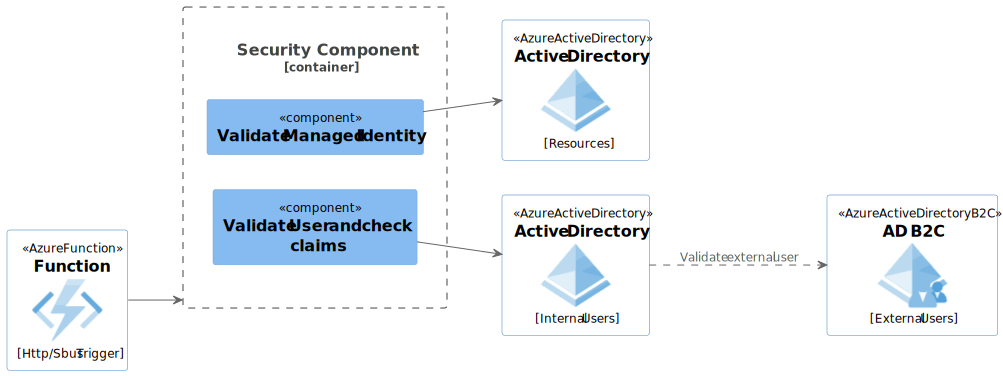
\includegraphics[keepaspectratio]{index_files/mediabag/SecurityComponent.png}}

}

\caption{image}

\end{figure}%

\begin{Shaded}
\begin{Highlighting}[]
\NormalTok{@startuml System
}
\NormalTok{{-}{-} !include not found: \textless{}C4/C4\_Component\textgreater{}
}
\NormalTok{{-}{-} !include not found: \textless{}azure/AzureCommon\textgreater{}
}
\NormalTok{{-}{-} !include not found: \textless{}azure/Compute/AzureFunction\textgreater{}
}
\NormalTok{{-}{-} !include not found: \textless{}azure/Web/AzureAPIManagement\textgreater{}
}
\NormalTok{{-}{-} !include not found: \textless{}azure/Integration/AzureServiceBusTopic\textgreater{}
}
\NormalTok{{-}{-} !include not found: \textless{}azure/Identity/all\textgreater{}
}

\NormalTok{LAYOUT\_LEFT\_RIGHT()
}

\NormalTok{        AzureActiveDirectory( adp, "Active Directory", "Resources")
}
\NormalTok{        AzureActiveDirectory( ad, "Active Directory", "Internal Users")
}
\NormalTok{        AzureActiveDirectoryB2C( b2c, "AD B2C", "External Users")
}
\NormalTok{        AzureFunction(aFunc, "Function", "Http/Sbus Trigger")
}
\NormalTok{        Container\_Boundary(sec, "Security Component", "Validates Calling service and users") \{
}
\NormalTok{            Component( mi, "Validate Managed Identity", "")
}
\NormalTok{            Component( us, "Validate User and check claims", "")
}

\NormalTok{        \}
}

\NormalTok{        ad ..\textgreater{} b2c : Validate external user
}
\NormalTok{        mi {-}{-}\textgreater{} adp 
}
\NormalTok{        us {-}{-}\textgreater{} ad 
}
\NormalTok{        aFunc {-}{-}\textgreater{} sec
}

\NormalTok{@enduml
}
\end{Highlighting}
\end{Shaded}

\section{Managed Identity}\label{managed-identity}

The Header of any incoming message will contain 2 header keys
\textbf{IDENTITY\_ENDPOINT} and \textbf{IDENTITY\_HEADER} they sometimes
appear under there alias names \textbf{MSI\_ENDPOINT} and
\textbf{MSI\_HEADER}.

\subsection{Retrieve the MI token}\label{retrieve-the-mi-token}

Use the DefaultAzureCredential to obtain the token for the managed
identity.

\begin{Shaded}
\begin{Highlighting}[]
\DataTypeTok{var}\NormalTok{ credential }\OperatorTok{=} \KeywordTok{new} \FunctionTok{DefaultAzureCredential}\OperatorTok{();}
\DataTypeTok{var}\NormalTok{ token }\OperatorTok{=}\NormalTok{ await credential}\OperatorTok{.}\FunctionTok{GetTokenAsync}\OperatorTok{(}\KeywordTok{new} \FunctionTok{TokenRequestContext}\OperatorTok{(}\KeywordTok{new}\OperatorTok{[]} \OperatorTok{\{} \StringTok{"https://management.azure.com/.default"} \OperatorTok{\}));}
\end{Highlighting}
\end{Shaded}

\subsection{Validate the token}\label{validate-the-token}

Use the Microsoft.IdentityModel.Tokens library to validate the token.
This involves checking the token's signature, issuer, audience, and
expiration.

\begin{Shaded}
\begin{Highlighting}[]
\KeywordTok{using}\NormalTok{ Microsoft}\OperatorTok{.}\FunctionTok{IdentityModel}\OperatorTok{.}\FunctionTok{Tokens}\OperatorTok{;}
\KeywordTok{using}\NormalTok{ System}\OperatorTok{.}\FunctionTok{IdentityModel}\OperatorTok{.}\FunctionTok{Tokens}\OperatorTok{.}\FunctionTok{Jwt}\OperatorTok{;}

\KeywordTok{public} \DataTypeTok{bool} \FunctionTok{ValidateToken}\OperatorTok{(}\DataTypeTok{string}\NormalTok{ token}\OperatorTok{)}
\OperatorTok{\{}
    \DataTypeTok{var}\NormalTok{ tokenHandler }\OperatorTok{=} \KeywordTok{new} \FunctionTok{JwtSecurityTokenHandler}\OperatorTok{();}
    \DataTypeTok{var}\NormalTok{ validationParameters }\OperatorTok{=} \KeywordTok{new}\NormalTok{ TokenValidationParameters}
    \OperatorTok{\{}
\NormalTok{        ValidateIssuer }\OperatorTok{=} \KeywordTok{true}\OperatorTok{,}
\NormalTok{        ValidIssuer }\OperatorTok{=} \StringTok{"https://sts.windows.net/\{tenant{-}id\}/"}\OperatorTok{,}
\NormalTok{        ValidateAudience }\OperatorTok{=} \KeywordTok{true}\OperatorTok{,}
\NormalTok{        ValidAudience }\OperatorTok{=} \StringTok{"https://management.azure.com/"}\OperatorTok{,}
\NormalTok{        ValidateLifetime }\OperatorTok{=} \KeywordTok{true}\OperatorTok{,}
\NormalTok{        IssuerSigningKeyResolver }\OperatorTok{=} \OperatorTok{(}\NormalTok{token}\OperatorTok{,}\NormalTok{ securityToken}\OperatorTok{,}\NormalTok{ kid}\OperatorTok{,}\NormalTok{ parameters}\OperatorTok{)} \OperatorTok{=\textgreater{}}
        \OperatorTok{\{}
            \CommentTok{// Retrieve signing keys from Azure AD}
            \DataTypeTok{var}\NormalTok{ discoveryDocument }\OperatorTok{=} \StringTok{"https://login.microsoftonline.com/\{tenant{-}id\}/v2.0/.well{-}known/openid{-}configuration"}\OperatorTok{;}
            \DataTypeTok{var}\NormalTok{ keys }\OperatorTok{=} \KeywordTok{new} \FunctionTok{JsonWebKeySet}\OperatorTok{(}\NormalTok{discoveryDocument}\OperatorTok{).}\FunctionTok{GetSigningKeys}\OperatorTok{();}
            \KeywordTok{return}\NormalTok{ keys}\OperatorTok{;}
        \OperatorTok{\}}
    \OperatorTok{\};}

    \KeywordTok{try}
    \OperatorTok{\{}
\NormalTok{        tokenHandler}\OperatorTok{.}\FunctionTok{ValidateToken}\OperatorTok{(}\NormalTok{token}\OperatorTok{,}\NormalTok{ validationParameters}\OperatorTok{,} \KeywordTok{out}\NormalTok{ SecurityToken validatedToken}\OperatorTok{);}
        \KeywordTok{return} \KeywordTok{true}\OperatorTok{;}
    \OperatorTok{\}}
    \KeywordTok{catch}
    \OperatorTok{\{}
        \KeywordTok{return} \KeywordTok{false}\OperatorTok{;}
    \OperatorTok{\}}
\OperatorTok{\}}
\end{Highlighting}
\end{Shaded}

\subsection{Authorise the caller}\label{authorise-the-caller}

Ensure the caller's managed identity has the necessary permissions to
access the function. This can be done by checking the claims in the
token.

\begin{Shaded}
\begin{Highlighting}[]
\DataTypeTok{var}\NormalTok{ jwtToken }\OperatorTok{=}\NormalTok{ tokenHandler}\OperatorTok{.}\FunctionTok{ReadJwtToken}\OperatorTok{(}\NormalTok{token}\OperatorTok{);}
\DataTypeTok{var}\NormalTok{ claims }\OperatorTok{=}\NormalTok{ jwtToken}\OperatorTok{.}\FunctionTok{Claims}\OperatorTok{;}

\CommentTok{// Check for specific roles or permissions}
\DataTypeTok{var}\NormalTok{ hasAccess }\OperatorTok{=}\NormalTok{ claims}\OperatorTok{.}\FunctionTok{Any}\OperatorTok{(}\NormalTok{c }\OperatorTok{=\textgreater{}}\NormalTok{ c}\OperatorTok{.}\FunctionTok{Type} \OperatorTok{==} \StringTok{"roles"} \OperatorTok{\&\&}\NormalTok{ c}\OperatorTok{.}\FunctionTok{Value} \OperatorTok{==} \StringTok{"YourRequiredRole"}\OperatorTok{);}
\end{Highlighting}
\end{Shaded}

\subsection{Function Code}\label{function-code}

By combining the above snippets, you would be able to check and
authorise the calling application.

\begin{Shaded}
\begin{Highlighting}[]
\KeywordTok{public} \KeywordTok{static}\NormalTok{ async Task}\OperatorTok{\textless{}}\NormalTok{IActionResult}\OperatorTok{\textgreater{}} \FunctionTok{Run}\OperatorTok{(}\NormalTok{HttpRequest req}\OperatorTok{,}\NormalTok{ ILogger log}\OperatorTok{)}
\OperatorTok{\{}
    \DataTypeTok{var}\NormalTok{ token }\OperatorTok{=}\NormalTok{ req}\OperatorTok{.}\FunctionTok{Headers}\OperatorTok{[}\StringTok{"Authorization"}\OperatorTok{].}\FunctionTok{ToString}\OperatorTok{().}\FunctionTok{Replace}\OperatorTok{(}\StringTok{"Bearer "}\OperatorTok{,} \StringTok{""}\OperatorTok{);}
    \KeywordTok{if} \OperatorTok{(!}\FunctionTok{ValidateToken}\OperatorTok{(}\NormalTok{token}\OperatorTok{))}
    \OperatorTok{\{}
        \KeywordTok{return} \KeywordTok{new} \FunctionTok{UnauthorizedResult}\OperatorTok{();}
    \OperatorTok{\}}

    \CommentTok{// Proceed with your function logic}
    \KeywordTok{return} \KeywordTok{new} \FunctionTok{OkResult}\OperatorTok{();}
\OperatorTok{\}}
\end{Highlighting}
\end{Shaded}

\section{User Authentication}\label{user-authentication}

\textbf{N.B. If a User token is included in the header then check the
user is authorised.}

Use the Microsoft.Identity.Web library to handle authentication and
authorization in your function.

\begin{Shaded}
\begin{Highlighting}[]
\KeywordTok{using}\NormalTok{ Microsoft}\OperatorTok{.}\FunctionTok{AspNetCore}\OperatorTok{.}\FunctionTok{Mvc}\OperatorTok{;}
\KeywordTok{using}\NormalTok{ Microsoft}\OperatorTok{.}\FunctionTok{Azure}\OperatorTok{.}\FunctionTok{WebJobs}\OperatorTok{;}
\KeywordTok{using}\NormalTok{ Microsoft}\OperatorTok{.}\FunctionTok{Azure}\OperatorTok{.}\FunctionTok{WebJobs}\OperatorTok{.}\FunctionTok{Extensions}\OperatorTok{.}\FunctionTok{Http}\OperatorTok{;}
\KeywordTok{using}\NormalTok{ Microsoft}\OperatorTok{.}\FunctionTok{AspNetCore}\OperatorTok{.}\FunctionTok{Http}\OperatorTok{;}
\KeywordTok{using}\NormalTok{ Microsoft}\OperatorTok{.}\FunctionTok{Extensions}\OperatorTok{.}\FunctionTok{Logging}\OperatorTok{;}
\KeywordTok{using}\NormalTok{ Microsoft}\OperatorTok{.}\FunctionTok{Identity}\OperatorTok{.}\FunctionTok{Web}\OperatorTok{;}
\KeywordTok{using}\NormalTok{ System}\OperatorTok{.}\FunctionTok{Threading}\OperatorTok{.}\FunctionTok{Tasks}\OperatorTok{;}

\KeywordTok{public} \KeywordTok{static} \KeywordTok{class}\NormalTok{ MyFunction}
\OperatorTok{\{}
    \OperatorTok{[}\FunctionTok{FunctionName}\OperatorTok{(}\StringTok{"MyFunction"}\OperatorTok{)]}
    \KeywordTok{public} \KeywordTok{static}\NormalTok{ async Task}\OperatorTok{\textless{}}\NormalTok{IActionResult}\OperatorTok{\textgreater{}} \FunctionTok{Run}\OperatorTok{(}
        \OperatorTok{[}\FunctionTok{HttpTrigger}\OperatorTok{(}\NormalTok{AuthorizationLevel}\OperatorTok{.}\FunctionTok{Function}\OperatorTok{,} \StringTok{"get"}\OperatorTok{,} \StringTok{"post"}\OperatorTok{,}\NormalTok{ Route }\OperatorTok{=} \KeywordTok{null}\OperatorTok{)]}\NormalTok{ HttpRequest req}\OperatorTok{,}
\NormalTok{        ILogger log}\OperatorTok{)}
    \OperatorTok{\{}
        \DataTypeTok{var}\NormalTok{ user }\OperatorTok{=}\NormalTok{ req}\OperatorTok{.}\FunctionTok{HttpContext}\OperatorTok{.}\FunctionTok{User}\OperatorTok{;}

        \KeywordTok{if} \OperatorTok{(!}\NormalTok{user}\OperatorTok{.}\FunctionTok{Identity}\OperatorTok{.}\FunctionTok{IsAuthenticated}\OperatorTok{)}
        \OperatorTok{\{}
            \KeywordTok{return} \KeywordTok{new} \FunctionTok{UnauthorizedResult}\OperatorTok{();}
        \OperatorTok{\}}

        \CommentTok{// Check for specific roles or claims}
        \KeywordTok{if} \OperatorTok{(!}\NormalTok{user}\OperatorTok{.}\FunctionTok{IsInRole}\OperatorTok{(}\StringTok{"YourRequiredRole"}\OperatorTok{))}
        \OperatorTok{\{}
            \KeywordTok{return} \KeywordTok{new} \FunctionTok{ForbidResult}\OperatorTok{();}
        \OperatorTok{\}}

        \CommentTok{// Proceed with your function logic}
        \KeywordTok{return} \KeywordTok{new} \FunctionTok{OkObjectResult}\OperatorTok{(}\StringTok{"User is authorized"}\OperatorTok{);}
    \OperatorTok{\}}
\OperatorTok{\}}
\end{Highlighting}
\end{Shaded}

\bookmarksetup{startatroot}

\chapter{Solution Strategy}\label{solution-strategy}

This solution follows the rules laid out in previous pattern
architecture documents.

\begin{longtable}[]{@{}
  >{\raggedright\arraybackslash}p{(\linewidth - 2\tabcolsep) * \real{0.2407}}
  >{\raggedright\arraybackslash}p{(\linewidth - 2\tabcolsep) * \real{0.7593}}@{}}
\toprule\noalign{}
\begin{minipage}[b]{\linewidth}\raggedright
Document
\end{minipage} & \begin{minipage}[b]{\linewidth}\raggedright
Link
\end{minipage} \\
\midrule\noalign{}
\endhead
\bottomrule\noalign{}
\endlastfoot
Third Party Integration &
\href{https://knightfrank.sharepoint.com/:w:/s/ArchitectureCentre/ERjTwYIlR9BNv3lC4iykBg0BWVgRoRwphJthTMNPbsKUvg?e=0Wjbn6}{Link} \\
Managed Identities &
\href{https://knightfrank.sharepoint.com/:w:/s/ArchitectureCentre/EaWEeNyofi1Np9jBidalZQcBOnq6ZXNjVVKi1Ds-qyHrIQ?e=FpScEF}{Link} \\
APIM &
\href{https://knightfrank.sharepoint.com/:w:/s/ArchitectureCentre/Eej7rqo7KPNFntrmKnBOZwIBewRFkiy74y1mM4Gnktp9rg?e=5eGwaH}{Link} \\
WebHooks &
\href{https://knightfrank.sharepoint.com/:w:/s/ArchitectureCentre/ESDumbDhct9OoV4owRF9-BIB99sTk8SqBV-ej916OY2xJQ?e=4GLqsJ}{Link} \\
Azure Functions &
\href{https://knightfrank.sharepoint.com/:w:/s/ArchitectureCentre/EartBoEkkIlPvdzS5xy2edABO5e9YJP9GzDrdpkC6kyIlg?e=DcOZz9}{Link} \\
Tenant, Subscribers and Resource Groups &
\href{https://knightfrank.sharepoint.com/:w:/s/ArchitectureCentre/ETIq1xmeohVEjFw-dOloBXsB6GnYgXwywAO2x_rDf6SYlw?e=b7HU2p}{Link} \\
\end{longtable}

\bookmarksetup{startatroot}

\chapter{Runtime View}\label{runtime-view}

\section{Overview}\label{overview-1}

This shows the general flow of how the system will function.

\begin{Shaded}
\begin{Highlighting}[]
\NormalTok{@startuml
}

\NormalTok{participant User as user
}
\NormalTok{participant Hub as hub
}
\NormalTok{database HubDB as db
}
\NormalTok{queue "Service Bus" as que
}
\NormalTok{participant Service as svc
}
\NormalTok{participant "Document Manager" as dm
}
\NormalTok{participant Frontify as fnt
}

\NormalTok{user {-}\textgreater{} hub 
}
\NormalTok{group Templates
}
\NormalTok{hub {-}\textgreater{} svc ++ \#gold: Get Templates
}
\NormalTok{svc {-}\textgreater{} fnt ++ \#gold: Get Templates
}
\NormalTok{fnt {-}{-}\textgreater{} svc {-}{-}
}
\NormalTok{svc {-}\textgreater{} fnt ++ \#gold: Get Template Details
}
\NormalTok{fnt {-}{-}\textgreater{} svc {-}{-}
}
\NormalTok{svc {-}{-}\textgreater{} hub {-}{-}
}
\NormalTok{end
}

\NormalTok{hub {-}\textgreater{} hub ++ \#gold: Prepare Text and Images
}

\NormalTok{hub {-}\textgreater{} que  ++ \#gold : Publish Brochure Artifacts 
}
\NormalTok{hub {-}{-}\textgreater{} user {-}{-}:done
}

\NormalTok{    que {-}\textgreater{} svc ++ \#gold: Subscribe
}
\NormalTok{loop
}
\NormalTok{        svc {-}\textgreater{} fnt ++ \#gold: Load artifacts
}
\NormalTok{        fnt {-}{-}\textgreater{} svc {-}{-}
}
\NormalTok{end
}
\NormalTok{        svc {-}\textgreater{} fnt ++ \#gold : Generate Brochure
}
\NormalTok{        fnt {-}{-}\textgreater{} svc {-}{-} : 
}
\NormalTok{        svc {-}\textgreater{} dm ++ \#gold: Store
}
\NormalTok{        dm {-}{-}\textgreater{} svc {-}{-}: Saved
}
\NormalTok{    svc {-}\textgreater{} que {-}{-}: Publish
}
\NormalTok{hub \textless{}{-} que {-}{-}++ \#gold: Subscribe Brochure Metadata
}
\NormalTok{hub {-}\textgreater{} db : Add Brochure to attachments
}
\NormalTok{hub {-}{-}\textgreater{} user {-}{-}: Notify
}

\NormalTok{====
}

\NormalTok{user {-}\textgreater{} hub ++ \#gold
}
\NormalTok{hub {-}\textgreater{} dm ++ \#gold: Access Brochure
}
\NormalTok{dm {-}{-}\textgreater{} hub {-}{-}: 
}
\NormalTok{hub {-}{-}\textgreater{} user
}

\NormalTok{@enduml
}
\end{Highlighting}
\end{Shaded}

\begin{enumerate}
\def\labelenumi{\arabic{enumi}.}
\tightlist
\item
  The selects if they want to generate a Bespoke or a Auto Generated
  brochure.
\item
  The service will make a Get Template request to Frontify, and filter
  the list to only those templates that are either the CSV or the Auto
  Generation brochure types.
\item
  The Get Templates method will return the template name and its detail.
\item
  Hub will create a service request object, and map the text and image
  artifacts to the template detail Keys.
\item
  Hub publishes the Brochure Generation request to the service bus.
\item
  The service picks up the brochure generation request, and creates a
  brochure object in the datastore.
\item
  If the User requested a Bespoke brochure then

  \begin{enumerate}
  \def\labelenumii{\arabic{enumii}.}
  \tightlist
  \item
    A CSV file is created.
  \item
    All of the image objects from the existing request brochure object
    are loaded into frontify and Assets are created.
  \item
    The Text and Asset Id's are written to the CSV.
  \item
    A request is made to the datastore to return all incomplete brochure
    objects.
  \item
    CSV rows are created for each.
  \item
    The CSV is uploaded.
  \item
    Once the Brochure has been created by the Frontify User, They will
    need to login to Hub and Upload the brochure, and indicate the
    generation is complete.

    \begin{enumerate}
    \def\labelenumiii{\arabic{enumiii}.}
    \tightlist
    \item
      Hub will inform the service that the brochure is complete.
    \item
      The service will complete the message in the datastore, stopping
      its inclusion in future CSV files.
    \end{enumerate}
  \end{enumerate}
\item
  If the User requested a Auto Generation Brochure then

  \begin{enumerate}
  \def\labelenumii{\arabic{enumii}.}
  \tightlist
  \item
    A Export Creative request is generated
  \item
    Either Poll Or Wait for a Webhook, which will indicate the
    generation is complete.
  \item
    Save the brochure in the Document Manager.
  \item
    Create a response message, and publish it onto the service bus.
  \end{enumerate}
\end{enumerate}

\bookmarksetup{startatroot}

\chapter{Deployment View}\label{deployment-view}

\begin{figure}[H]

{\centering \pandocbounded{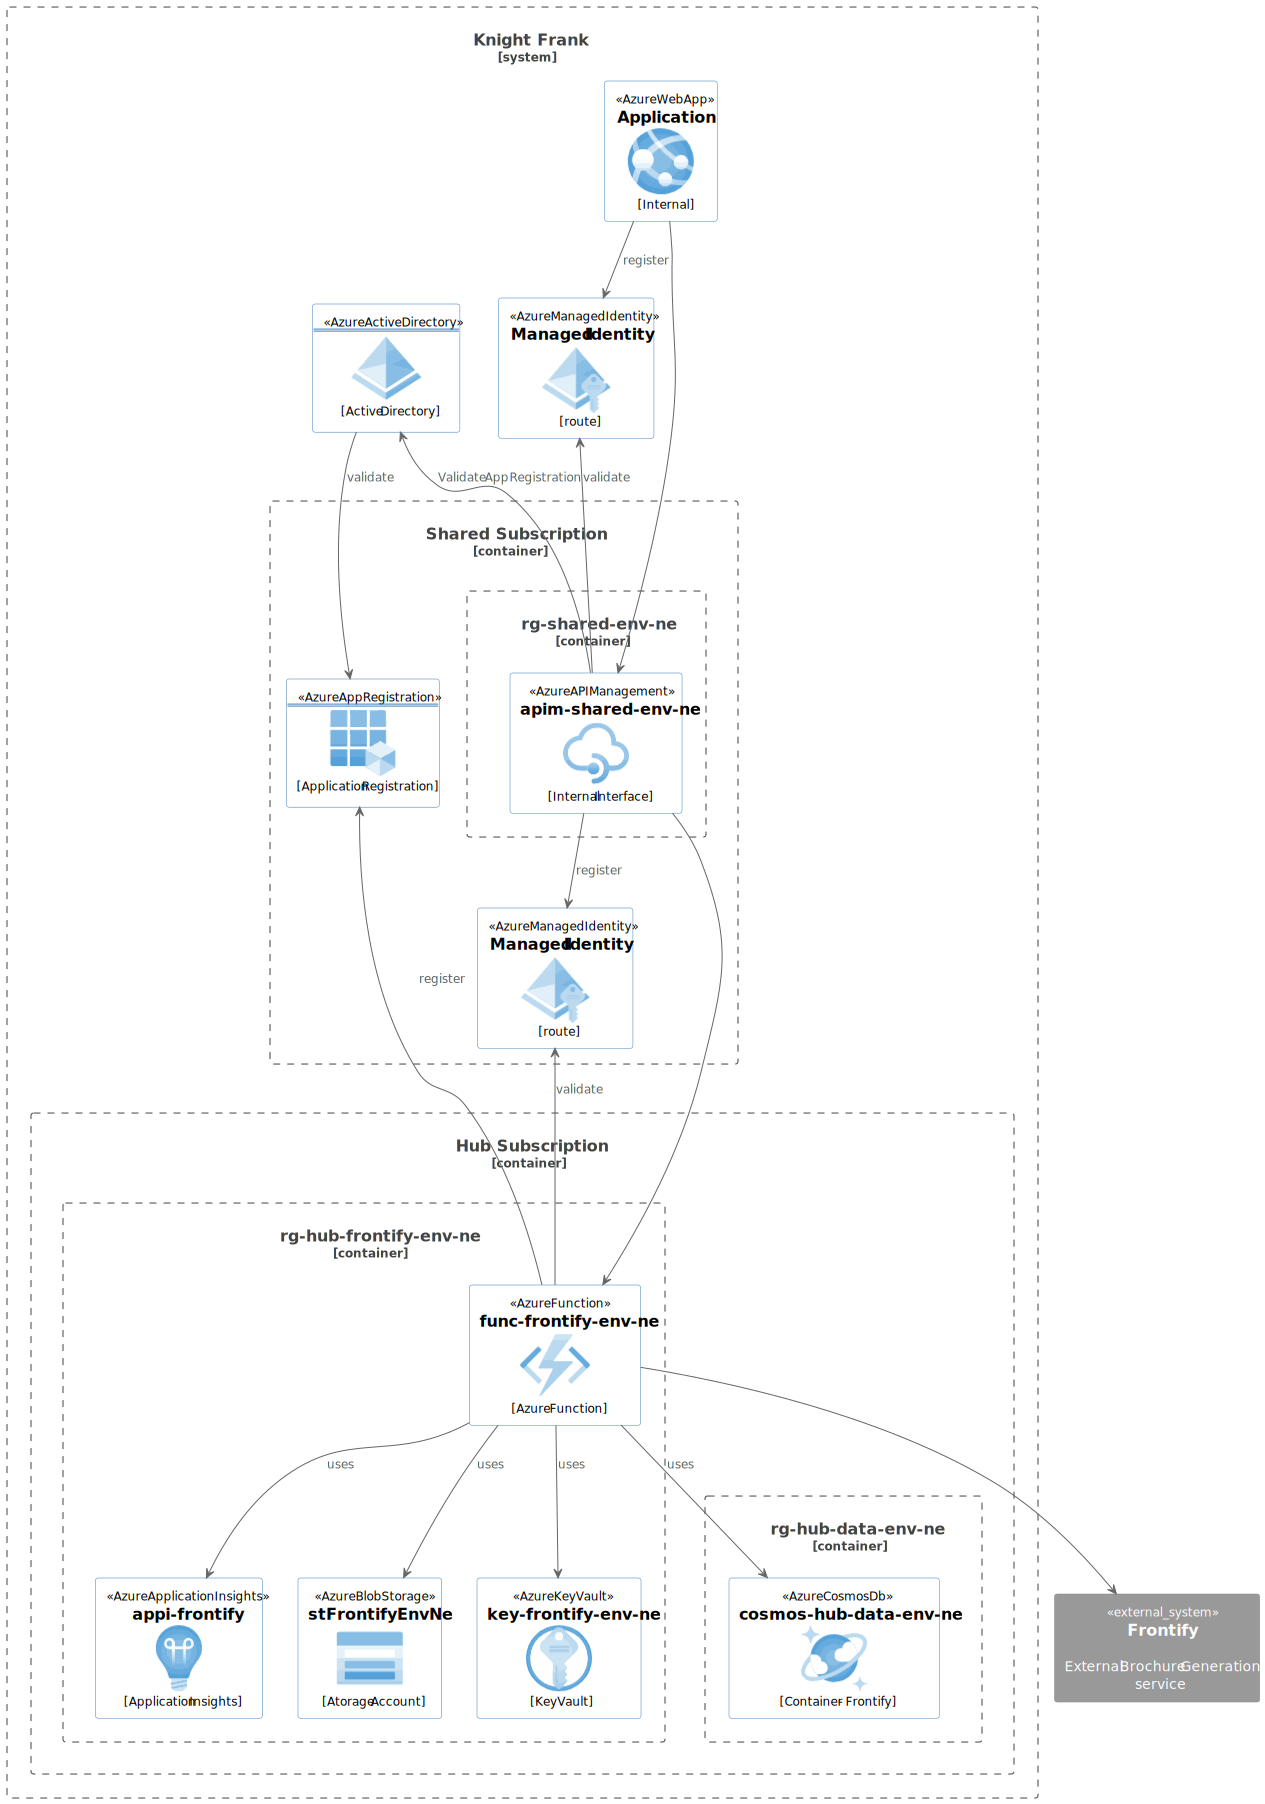
\includegraphics[keepaspectratio]{index_files/mediabag/DeploymentView.png}}

}

\caption{image}

\end{figure}%

\begin{Shaded}
\begin{Highlighting}[]
\NormalTok{@startuml DeploymentView
}
\NormalTok{{-}{-} !include not found: \textless{}C4/C4\_Component\textgreater{}
}
\NormalTok{{-}{-} !include not found: \textless{}azure/AzureCommon\textgreater{}
}
\NormalTok{{-}{-} !include not found: \textless{}azure/Compute/AzureFunction\textgreater{}
}
\NormalTok{{-}{-} !include not found: \textless{}azure/Web/AzureAPIManagement\textgreater{}
}
\NormalTok{{-}{-} !include not found: \textless{}azure/Integration/AzureServiceBusTopic\textgreater{}
}
\NormalTok{{-}{-} !include not found: \textless{}azure/Networking/AzureApplicationGateway\textgreater{}
}
\NormalTok{{-}{-} !include not found: \textless{}azure/Networking/All\textgreater{}
}
\NormalTok{{-}{-} !include not found: \textless{}azure/Web/AzureWebApp\textgreater{}
}
\NormalTok{{-}{-} !include not found: \textless{}azure/DevOps/AzureApplicationInsights\textgreater{}
}
\NormalTok{{-}{-} !include not found: \textless{}azure/Storage/AzureBlobStorage\textgreater{}
}
\NormalTok{{-}{-} !include not found: \textless{}azure/Databases/AzureCosmosDb\textgreater{}
}
\NormalTok{{-}{-} !include not found: \textless{}azure/Security/AzureKeyVault\textgreater{}
}
\NormalTok{{-}{-} !include not found: \textless{}azure/Identity/AzureAppRegistration\textgreater{}
}
\NormalTok{{-}{-} !include not found: \textless{}azure/Identity/AzureActiveDirectory\textgreater{}
}
\NormalTok{{-}{-} !include not found: \textless{}azure/Identity/AzureManagedIdentity\textgreater{}
}

\NormalTok{\textquotesingle{}LAYOUT\_WITH\_LEGEND()
}
\NormalTok{\textquotesingle{}LAYOUT\_LEFT\_RIGHT()
}

\NormalTok{AddElementTag("microService", $shape=EightSidedShape(), $fontColor="white", $legendText="micro service\textbackslash{}neight sided")
}
\NormalTok{AddElementTag("storage", $shape=RoundedBoxShape(), $fontColor="white")
}

\NormalTok{System\_Boundary(s1, "Knight Frank") \{
}

\NormalTok{    AzureWebApp(local, "Application", "Internal")
}
\NormalTok{    AzureActiveDirectory(ad, "", "Active Directory")
}
\NormalTok{    AzureManagedIdentity(miapp, "Managed Identity", "route")
}

\NormalTok{    Container\_Boundary(c1, "Shared Subscription") \{
}

\NormalTok{        Container\_Boundary(rgsh, "rg{-}shared{-}env{-}ne") \{
}
\NormalTok{            AzureAPIManagement(apimI, "apim{-}shared{-}env{-}ne", "Internal Interface")
}
\NormalTok{            apimI {-}up{-}\textgreater{} ad : Validate App Registration
}
\NormalTok{        \}
}

\NormalTok{        AzureManagedIdentity(misvc, "Managed Identity", "route")
}
\NormalTok{        AzureAppRegistration(reg, "", "Application Registration")
}

\NormalTok{    \}
}
    
\NormalTok{    Container\_Boundary(c2, "Hub Subscription") \{
}
\NormalTok{        Container\_Boundary(rggw, "rg{-}hub{-}frontify{-}env{-}ne") \{
}
\NormalTok{            AzureFunction(svc, "func{-}frontify{-}env{-}ne", "Azure Function")
}
\NormalTok{            AzureApplicationInsights(ai, "appi{-}frontify", "Application Insights")
}
\NormalTok{            AzureBlobStorage(st, "stFrontifyEnvNe", "Atorage Account")
}
\NormalTok{            AzureKeyVault(key, "key{-}frontify{-}env{-}ne", "Key Vault")
}

\NormalTok{            svc {-}{-}\textgreater{} ai : uses
}
\NormalTok{            svc {-}{-}\textgreater{} st : uses
}
\NormalTok{            svc {-}{-}\textgreater{} key : uses
}
\NormalTok{            svc {-}up{-}\textgreater{} reg : register
}
\NormalTok{        \}
}

\NormalTok{        Container\_Boundary(rgsd, "rg{-}hub{-}data{-}env{-}ne") \{
}
\NormalTok{            AzureCosmosDb(db, "cosmos{-}hub{-}data{-}env{-}ne", "Container {-} Frontify")
}
\NormalTok{        \}
}

\NormalTok{        svc {-}{-}\textgreater{} db : uses
}
\NormalTok{        apimI {-}\textgreater{} svc 
}
\NormalTok{        local {-}{-}{-}\textgreater{} apimI
}

\NormalTok{        apimI {-}down{-}\textgreater{} misvc : register
}
\NormalTok{        svc {-}up{-}\textgreater{} misvc : validate
}
\NormalTok{    \}
}

\NormalTok{    rgsh {-}[hidden]{-} rggw
}
\NormalTok{    rgsh {-}[hidden]{-} rgsd
}

\NormalTok{    local {-}down{-}\textgreater{} miapp : register
}
\NormalTok{    apimI {-}up{-}\textgreater{} miapp : validate
}
\NormalTok{    ad {-}down{-}\textgreater{} reg : validate
}

\NormalTok{\}
}

\NormalTok{System\_Ext(extFrontify, "Frontify", "External Brochure Generation service")
}
\NormalTok{svc {-}{-}\textgreater{} extFrontify
}

\NormalTok{@enduml
}
\end{Highlighting}
\end{Shaded}

\section{Security}\label{security}

The application is accessed by Internal web applications.

\begin{itemize}
\tightlist
\item
  Internal are within the companies network.
\item
  Not accessible from the public internet.
\item
  Managed Identity will be used between APIM and the Azure Function
  Service.
\item
  The Azure Function will validate the MI token.
\end{itemize}

\section{Application}\label{application}

\begin{itemize}
\tightlist
\item
  The Application resource group will contain the usual components for a
  microservice.
\item
  The components will follow our naming convention.
\end{itemize}

\begin{longtable}[]{@{}
  >{\raggedright\arraybackslash}p{(\linewidth - 4\tabcolsep) * \real{0.2326}}
  >{\raggedright\arraybackslash}p{(\linewidth - 4\tabcolsep) * \real{0.2326}}
  >{\raggedright\arraybackslash}p{(\linewidth - 4\tabcolsep) * \real{0.5349}}@{}}
\toprule\noalign{}
\begin{minipage}[b]{\linewidth}\raggedright
Component
\end{minipage} & \begin{minipage}[b]{\linewidth}\raggedright
Name
\end{minipage} & \begin{minipage}[b]{\linewidth}\raggedright
\end{minipage} \\
\midrule\noalign{}
\endhead
\bottomrule\noalign{}
\endlastfoot
Azure Function & func-frontify-env-ne & \\
Application Insights & appi-frontify-env-ne & \\
Storage Account & stfrontifyEnvNe & Camelcase for readability, should be
lowercase \\
Key Vault & key-frontify-env-ne & \\
\end{longtable}

\textbf{N.B. Env should be changed to match the deployment environment.}

The Application will be registered in Active Directory (Entra).

\section{DataStore.}\label{datastore.}

\begin{itemize}
\tightlist
\item
  The application uses a Cosmos Database as its data store.
\item
  A new cosmos DB container of NOSQL type should be set up.
\end{itemize}




\end{document}
